\documentclass[11pt]{article}

% ---------------------------------------------------------------------
% Standard packages
% ---------------------------------------------------------------------
\usepackage[margin=1in]{geometry}       % Adjust margins cleanly
\usepackage[utf8]{inputenc}             % Proper encoding
\usepackage[T1]{fontenc}                % Better font encoding
\usepackage{setspace}                   % For line spacing if needed

% ---------------------------------------------------------------------
% Math and symbols
% ---------------------------------------------------------------------
\usepackage{amsmath, amssymb, amsfonts, mathtools}
\usepackage{mathrsfs}                   % Script math fonts

% ---------------------------------------------------------------------
% Figures and tables
% ---------------------------------------------------------------------
\usepackage{graphicx}                   % For including graphics
\usepackage{subcaption}                 % For subfigures
\usepackage{booktabs, threeparttable}   % For nice tables
\usepackage{multirow, array}            % For complex table layouts
\usepackage{caption}                    % Custom caption formatting
\usepackage{float}                      % Better float handling
\usepackage{changepage}                 % For adjusting table/figure widths

% ---------------------------------------------------------------------
% Colors and highlighting
% ---------------------------------------------------------------------
\usepackage{xcolor, soul}

% ---------------------------------------------------------------------
% References / citations
% ---------------------------------------------------------------------
\usepackage[authoryear,round]{natbib}   % Author-year citation style
\bibliographystyle{apalike}             % APA-like reference formatting

% ---------------------------------------------------------------------
% Misc
% ---------------------------------------------------------------------
\usepackage{url}                        % For URLs in references

% ---------------------------------------------------------------------
% Line spacing and paragraph spacing
% ---------------------------------------------------------------------
\setstretch{1.2}                        % Adjust line spacing (e.g., 1.2)
\setlength{\parskip}{0.8em}             % Add space between paragraphs
\setlength{\parindent}{0pt}             % No paragraph indentation

\usepackage{fancyhdr}
\DeclareMathAlphabet{\mathpzc}{OT1}{pzc}{m}{it} \DeclareMathAlphabet{\mathfrak}{U}{euf}{m}{n}
 \vspace{5mm} \setlength{\topmargin}{-.5in} \setlength{\textheight}{8.85in}
\setlength{\oddsidemargin}{-.02in} \setlength{\textwidth}{6.6in}
\parskip.10in
\newtheorem{example}{Example}
\newtheorem{theorem}{Theorem}
\newtheorem{lemma}{Lemma}
\newtheorem{claim}{Claim}
\newtheorem{corollary}{Corollary}
\newtheorem{proposition}{Proposition}
\def\proof{\noindent{\bf Proof.}}
%\def\QED{\hfill{$\rule{6pt}{6pt}$} \newline}
%\def\qed{\hfill{$\rule{6pt}{6pt}$} \newline}
\newcommand{\remove}[1]{}
\newenvironment{quote1}
{\begin{list}
         {\setlength{\leftmargin}{1.0in}}
         {\setlength{\rightmargin}{0.25in}}
         \small
         \baselineskip=14pt
         \item[]
}{\end{list}}
\newenvironment{quote2}
{ \bigskip
\noindent
         \small\em
         \baselineskip=14pt
}





%\input setps

\newcommand{\teq}{\triangleq}
\newcommand{\E}{\mathbb E}
\newcommand{\N}{\mathbb N}
\newcommand{\F}{\cal F}
\newcommand{\1}{\hbox{\rm 1\kern-.35em 1}}
% Private macros here (check that there is no clash with the style)
\newcommand{\un}{\underline}
\newcommand{\ov}{\overline}
\newcommand{\MD}{\mathscr D}
\newcommand{\MT}{\mathscr T}
\pagenumbering{arabic}



\begin{document}
% \font\ex=msam10 at 10 pt \font\eu=eurb10 at 11 pt \font\ep=MSBM10 at 11 pt \LARGE
\setlength{\parindent}{0pt}
\pagestyle{fancy}
\fancyhead{}
\fancyhead[RO,RE]{\small{General Response \& Summary of Main Changes}}
\renewcommand{\headrulewidth}{0.0pt}

\begin{center}
{Authors' Response to Review of Manuscript MS-HCM-2025-01252}

\vspace{1mm}
\Large
\textbf{The Impact of Batching Advanced Imaging Tests\\ in Emergency Departments}
\vspace{1mm}

\end{center}
 \pagenumbering{arabic}
 \normalsize
\baselineskip=16pt
\noindent\underline{\textbf{I. General Response to the Entire Review Team}}



\noindent We would like to thank the Associate Editor (AE) and the three referees for the constructive and detailed feedback provided in their reports. We are also grateful for the opportunity to address the reviewers' comments, and for the revision decision.

We have carefully revised the paper to address all the comments, and the paper has benefited greatly from the suggested revisions. We first briefly summarize the main changes and then provide individual responses.

\begin{enumerate}
\item We have addressed the remaining methdological suggestions by the reviewers, including...
\item Throughout the paper...
\end{enumerate}


We hope the review team finds our various efforts in extending our results, and in carefully addressing the comments, satisfactory in this round.






%%%%%%%%%%%%%%%%%%%%%%%%%%%%%%%%%%%%%%%%%%%%%%%%%%%%%%%%%%%%%%%%%%%%%%%%%%%%%%%%%%%%%%%%%%%%%%%%%%%%%%%%%%%%%%%%%%%%%



\clearpage
%%%%%%%%%%%%%%%%%%%%%%%%%%%%%%%%%%%%%%%%%%%%%%%%%%%%%%%%%%%%%%%%%%%%%%%%%%%%%%
%%  SRESPONSES TO ASSOCIATE EDITOR (AE) COMMENTS              %%
%%%%%%%%%%%%%%%%%%%%%%%%%%%%%%%%%%%%%%%%%%%%%%%%%%%%%%%%%%%%%%%%%%%%%%%%%%%%%%

\pagestyle{fancy}
\fancyhead{}
\fancyhead[RO,RE]{\small{Responses to Associate Editor Comments}}
\renewcommand{\headrulewidth}{0.0pt}

\noindent\underline{\textbf{II. Responses to Associate Editor (AE) Comments}}

%%%%%%%%%%%%%%%%%%%%%%%%%%%  AE Comment 1  %%%%%%%%%%%%%%%%%%%%%%%%%%%%%%%%%%
\begin{quote2}
\textbf{AE Wrote (Overall assessment):} 

\noindent ``The study addresses an innovative and interesting research question, and the main finding is indeed surprising. On the surface, simultaneous ordering of diagnostic tests would appear to improve efficiency; this counterintuitive result raises important questions.

However, the referees have raised significant concerns regarding theory and methodology. In its current form, the paper does not sufficiently develop the theoretical foundation necessary to support its empirical strategy or claims of contribution.” 
\end{quote2}

\noindent\textbf{Response:} \textcolor{blue}{[Your response here]}

%%%%%%%%%%%%%%%%%%%%%%%%%%%  AE Comment 2  %%%%%%%%%%%%%%%%%%%%%%%%%%%%%%%%%%
\begin{quote2}
\textbf{AE Wrote (Comment – Theory needs clarification):}

\noindent ``The theoretical foundation requires significant clarification. Key questions remain unaddressed:
\begin{itemize}
 \item Is batching truly a disrectionary decision by the physician, or is it also driven by, perhaps unobserved clinical factors which affect ED LOS?
 \item Are additional tests medically required at the time of ordering, or are they preemptively ordered to buy time in anticipation of further needs?
 \item Could batching be a consequence of prior diagnostic uncertainty (e.g., pending results, routine requirements for referrals) or contextual factors such as utilization of the unit?"
\end{itemize}

Without a clearer articulation of the decision-making process and its drivers, the interpretation of the results remains ambiguous.

\end{quote2}

\noindent\textbf{Response:} 
\color{blue}
We appreciate the Associate Editor's request for theoretical clarification, which has led to substantial improvements in how we frame and interpret our study. We have made extensive revisions throughout the manuscript to address each of these important questions.

\textbf{1. Discretionary versus clinically-driven batching:} Our study isolates \textit{discretionary} batching decisions—those driven by physician practice style rather than clinical necessity—which is the precise margin where ED management can intervene. We establish this through our unique empirical setting and identification strategy:

First, Mayo Clinic's rotational patient assignment mechanism provides quasi-random assignment of patients to physicians. As documented by \cite{Traub2016; traub2016emergency; Traub2018}, patients are assigned to physicians through a computerized algorithm that is based solely on arrival time, without consideration of patient characteristics, complaint severity, or physician workload. This random assignment is crucial: it ensures that differences in batching rates across physicians reflect physician preferences rather than systematic differences in patient mix or unobserved clinical factors. Figure 2 provides empirical verification—while patient characteristics strongly predict batching decisions (left panel), they do not predict assignment to high versus low batch-tendency physicians (right panel), indicating that conditional on controls assignment to phsyician is as good as random.

Second, our LATE identifies effects specifically for ``compliers"—the fraction of patients whose batching decision changes depending on physician assignment. These patients, by definition, lack clear clinical indicators mandating either batching or sequential testing. They represent the discretionary margin where physician preference determines the testing strategy. The existence of these compliers demonstrates that discretionary batching exists and is substantial enough to matter for ED operations.

Third, we focus on \textit{early} batching (batching that occurs during the first test order) to capture decisions made before clinical information unfolds. At this moment of maximum uncertainty, some physicians opt for comprehensive imaging, while others maintain diagnostic flexibility. Late batching in response to test results occurs in only 1.91\% of multi-test encounters, confirming our focus on initial discretionary decisions rather than adaptive clinical responses.
Importantly, we do not claim all batching is discretionary. Some patients clearly require multiple urgent tests (the "always-takers"), while others need only a single test (the "never-takers"). Our contribution is identifying and quantifying the effects of discretionary batching for patients at the margin—precisely where ED protocols, decision support systems, and training interventions can influence practice without constraining necessary clinical judgment.

\textbf{2. Preemptive ordering and physician workflow management:} The existence of compliers in our analysis provides definitive evidence that discretionary batching occurs. If batching were driven purely by clinical necessity, we would observe minimal physician-induced variation—all physicians would batch for the same patients based on clinical presentation. Instead, our complier analysis (detailed in Appendix B) reveals that 13\% of patients receive batched imaging when assigned to high-tendency physicians but sequential testing when assigned to low-tendency physicians. These patients, by definition, lack clear clinical indicators mandating either approach.

The operational consequences of discretionary batching are unambiguous in our data. For these marginal patients, batching generates 1.4 additional imaging tests performed without improving diagnostic outcomes (72-hour return rates: -0.012, SE=0.018, p=0.50). While we cannot determine whether specific tests are clinically unnecessary, the pattern is clear: at the margin where physicians have discretion, batching increases resource utilization without measurable quality benefits.
Table 6 provides additional evidence that batching serves workflow management purposes. The significant decline in batching probability as shifts progress (-0.004 per hour, p<0.05) is inconsistent with clinical drivers, as patient acuity does not systematically vary by physician shift hour under Mayo Clinic's random assignment mechanism. This temporal pattern, combined with the attenuation of batching under major overcapacity conditions (Table 5), suggests physicians modulate their batching behavior based on operational context rather than purely clinical factors.

The 44.5 percentage point increase in admission probability warrants careful interpretation. Based on extensive consultation with our emergency medicine physician co-authors at both study sites, this pattern aligns with well-documented diagnostic cascades where additional imaging identifies incidental findings that, while not addressing the presenting complaint, trigger defensive admission decisions. The medical literature extensively documents this phenomenon (Ganguli et al., 2019; Hoffman \& Cooper, 2012).

Our contribution is precise: we quantify the operational impact of discretionary batching for patients at the margin where physician preference, rather than clinical protocols, determines the testing strategy. The reduced form estimates provide the causal effect of assignment to physicians with different batching tendencies. Even if some portion of this effect operates through channels beyond pure batching (potential exclusion restriction violations), the magnitude and consistency of effects across both study sites demonstrate that physician-induced variation in testing strategies creates substantial operational inefficiencies. These findings have direct policy relevance for the 13\% of patients whose care pathway depends on physician assignment—the precise population where ED protocols and training interventions can improve efficiency without constraining clinical autonomy.


\textbf{3. Diagnostic uncertainty and contextual factors:}
We carefully distinguish between clinically-appropriate responses to uncertainty and discretionary practice patterns. Our analysis reveals that discretionary batching—the type influenced by physician preference—varies with contextual factors in predictable ways:
Table 5 demonstrates that under major overcapacity, the frequency of discretionary batching drops (9.9\% vs. 15.8\% during normal operations) and its negative effects attenuate. The imaging increase falls from 1.36 to 1.16 tests, suggesting physicians become more selective when resources are constrained, eliminating discretionary batching while preserving clinically necessary batching.

Our heterogeneity analysis (Appendix C) shows that while batching rates vary across complaint types (31\% for trauma vs. 8\% for extremity complaints), the operational inefficiencies of discretionary batching persist across categories. This confirms that physician-induced batching—the variation our IV identifies—represents a suboptimal practice style rather than a clinically-tailored response to case complexity.

\color{black}
%%%%%%%%%%%%%%%%%%%%%%%%%%%  AE Comment 3  %%%%%%%%%%%%%%%%%%%%%%%%%%%%%%%%%%
\begin{quote2}
\textbf{AE Wrote (Comment – Empirical concerns):} 

\noindent``The observed effect with an increase of 130\% in ED stay as a result of batching is striking and, in fact, lacks credibility. Such a large effect increases the likelihood of confounding and therefore demands a very high degree of confidence in the empirical approach. As pointed out by several reviewers, there are unresolved concerns regarding the physician-patient assignment process. It is unclear whether this assignment is truly exogenous. For example, some physicians might only work certain shifts or treat specific patient types.

All reviewers were critical of the empirical strategy. Nevertheless, I believe the data offer enough potential to address these concerns through a substantial revision. This would require a significant improvement of both the theoretical development and the empirical analysis.

Based on the reviewers’ feedback and my own assessment, I believe there is a potential path toward eventual publication albeit at a very high risk. In addition to responding to the referee’s concerns, the revision needs to address the following key points:” 
\end{quote2}

\textbf{Response:} \color{blue}{We appreciate the Associate Editor's candid assessment and understand why the 130\% increase in ED length of stay appears striking at first glance. This skepticism motivated extensive robustness checks and clarification in the manuscript, which ultimately strengthened confidence in our findings. We have substantially revised both the theoretical foundation and empirical analysis to address these concerns.

\textbf{Addressing the magnitude of the effect:} While the 130\% increase appears substantial, it becomes more interpretable when broken down into its operational components. Our mediation analysis (Section 4.3) reveals that discretionary batching leads to 1.4 additional imaging tests for marginal patients. Given average imaging turnaround times in our data (90 minutes for non-contrast CT, 142 minutes for contrast CT, 165 minutes for ultrasound), these additional tests mechanically extend stays by 2-3 hours. Combined with the cognitive burden of processing multiple simultaneous results and the increased likelihood of admission (a 44.5 percentage point increase), the cumulative effect reaches the observed magnitude.

Importantly, this effect represents the Local Average Treatment Effect for the 13\% of patients who are compliers—those whose testing strategy changes based on physician assignment. These marginal patients often lack clear clinical protocols that dictate their imaging pathway, making them particularly susceptible to extended stays when subjected to comprehensive upfront testing rather than sequential evaluation.


\textbf{Establishing exogenous assignment:}
We have comprehensively addressed concerns about assignment exogeneity through multiple approaches:
First, the Mayo Clinic utilizes a computerized rotational assignment algorithm that assigns patients to physicians solely based on arrival order, without considering patient characteristics, complaint type, or physician workload. This system, documented in peer-reviewed publications (\cite{Traub2016, traub2016emergency, Traub2018}), removes discretion from the matching process. Section 3.1 now provides extensive detail about this mechanism, including how physicians receive four consecutive patients at shift start before entering rotation, and how the system caps physicians at 18 patients with no new assignments in their final 120 minutes.

Second, Figure 2 provides empirical verification of randomization. While patient characteristics strongly predict batching decisions (left panel), these same characteristics show no association with assignment to high versus low batch-tendency physicians (right panel). All coefficients are near zero with confidence intervals crossing zero, confirming that, conditional on shift fixed effects, assignment is effectively random.

Third, regarding the concern that some physicians might only work specific shifts, our fixed effects for day of week and time of day explicitly account for physician scheduling patterns. The residualized batch tendency measure captures physician-specific variation after removing these temporal patterns. Even if certain physicians systematically work different shifts, our approach ensures we identify variation within shift types.

\textbf{Robustness of empirical strategy:} Following all three reviewers' suggestions, we have implemented comprehensive robustness checks: 

\begin{itemize}
    \item Alternative instrument construction: Per Reviewer 3's suggestion, we constructed an alternative instrument using physician fixed effects directly (with leave-one-out correction). This approach yields virtually identical results (log LOS: 0.835 vs. 0.837), with a first-stage F-statistic of 187.

    \item Controls for correlated physician tendencies: We constructed measures of physician admission tendency and laboratory test ordering using the same methodology to control for correlated physician behaviors, which could be driving results (as mentioned by Reviewer 1). Including these controls yields minimal attenuation (log LOS: 0.837 → 0.821), indicating our instrument captures batching-specific variation rather than general physician characteristics.

    \item External validation: Replication at Massachusetts General Hospital, despite its different assignment mechanism and staffing model, yields remarkably similar effects (44.3\% increase in LOS, 1.8 additional tests). The consistency across institutions with different operational structures suggests our findings reflect fundamental inefficiencies of discretionary batching rather than institution-specific artifacts.


    \item Placebo and falsification tests: We find no effects of batch tendency on outcomes for patients with complaints where batching is clinically inappropriate (Appendix D). Additionally, batch tendency does not predict laboratory test ordering after controlling for patient characteristics, confirming specificity to imaging decisions.

\end{itemize}


\textbf{Improvements to theoretical development:} We have added Section 2.3, which includes formal hypothesis development, linking cognitive load theory and defensive medicine literature to predict batching behaviors. This theoretical framework clarifies that we study discretionary batching at the margin where physician style, rather than clinical necessity, determines testing strategy—precisely where ED interventions can improve efficiency.

\textbf{Strengthened empirical analysis:} Beyond the robustness checks above, we have:

\begin{itemize}
    \item Expanded sample selection documentation with a CONSORT diagram (Appendix Figure A2)
\item  Added heterogeneity analysis by complaint complexity (Appendix C)

\item  Included alternative outcome specifications suggested by R3 (treatment time, any 72-hour return)

\item Provided detailed complier characterization (Appendix B)

\end{itemize}

The convergence of evidence across multiple specifications, institutions, and methodological approaches provides the high degree of confidence the Associate Editor rightly demands. While the magnitude remains striking, it is empirically robust and operationally explicable, reflecting genuine inefficiencies when physicians exercise discretion to batch tests for patients lacking clear clinical protocols.

\color{black}

\begin{quote2}
\textbf{AE Wrote (Comment – Hypothesis development):} 

\noindent``The current framing does not clearly distinguish between “batching” and “sequencing” of diagnostic tests. A more precise hypothesis is needed. See also Ref 2 and Ref 3.” 

\end{quote2}

\noindent\textbf{Response:} \textcolor{blue}{[Your response here]}


\begin{quote2}
\textbf{AE Wrote (Comment – Outcome variable):} 

\noindent``Consider integrating intermediate outcomes / mechanisms, such as the order and type of tests performed. Are all tests necessary in each case? ED length of stay is a problematic outcome due to factors like patient heterogeneity, workload fluctuations, and staffing variability. The reviewer comments offer several suggestions here.” 

\end{quote2}

\noindent\textbf{Response:} \textcolor{blue}{[Your response here]}

\begin{quote2}
\textbf{AE Wrote (Comment – Relevance):} 

\begin{itemize}
    \item ``Focusing on subsets of patients or refining outcomes may help understand and explain the large effect size."
    \item ``A counterfactual cost-benefit analysis could strengthen the case for the practical relevance of the findings.” 
\end{itemize}

\end{quote2}

\noindent\textbf{Response:} \textcolor{blue}{[Your response here]}


\begin{quote2}
\textbf{AE Wrote (Comment – Additional suggestions):} 

\noindent``The following additional detailed suggestions could help the authors for developing the manuscript:

\begin{enumerate}
    \item Reassess the definition of the treatment variable (e.g. Ref 3).
    \item Examine the independence of test orders from prior tests and workload conditions (e.g. Ref 2).
    \item Include a section discussing sample representativeness.
    \item Expand the empirical strategy to address unobserved physician and non-physician factors. For instance, Ref 1 recommends using physician fixed effects. Also, reconsider model selection in light of the main outcome.
    \item Re-evaluate whether ED length of stay should remain the primary outcome. Alternative metrics such as time from test order to result may offer more insight."
\end{enumerate}

\end{quote2}

\noindent\textbf{Response:} \textcolor{blue}{[Your response here]}



%%%%%%%%%%%%%%%%%%%%%%%%%%%%%%%%%%%%%%%%%%%%%%%%%%%%%%%%%%%%%%%%%%%%%%%%%%%%%%
% End of AE responses
%%%%%%%%%%%%%%%%%%%%%%%%%%%%%%%%%%%%%%%%%%%%%%%%%%%%%%%%%%%%%%%%%%%%%%%%%%%%%%

\clearpage

%%%%%%%%%%%%%%%%%%%%%%%%%%%%%%%%%%%%%%%%%%%%%%%%%%%%%%%%%%%%%%%%%%%%%%%%%%%%%%
%%  SECTION IV – RESPONSES TO REVIEWER 1 COMMENTS                           %%
%%%%%%%%%%%%%%%%%%%%%%%%%%%%%%%%%%%%%%%%%%%%%%%%%%%%%%%%%%%%%%%%%%%%%%%%%%%%%%

\pagestyle{fancy}
\fancyhead{}
\fancyhead[RO,RE]{\small{Responses to Referee 1 Comments}}
\renewcommand{\headrulewidth}{0pt}

\noindent\underline{\textbf{III. Responses to Referee 1 (R1) Comments}}

%%%%%%%%%%%%%%%%%%%%%%%%%%%  R1 Comment 1  %%%%%%%%%%%%%%%%%%%%%%%%%%%%%%%%%%
\begin{quote2}
\textbf{R1 Wrote (Research question \& contribution):}  

\noindent``The research question is clear, and it is an important area of study. Emergency departments are
high-stress work environments where the stakes are high and patient lives are at stake.
Anything we can learn to improve the performance and outcomes of the work that is done there
could save lives, and also enhance our understanding of the impact of “work behavior /
preferences” on operational outcomes.” 
\end{quote2}

\noindent\textbf{***Response:} \textcolor{blue}{We sincerely appreciate the reviewer's recognition of the importance and clarity of our research question. We share your view that emergency departments represent uniquely high-stakes environments where operational improvements can have life-saving implications. Your framing of our work as contributing to the understanding of how ``work behavior/preferences" affect operational outcomes perfectly captures what we hope to achieve—bridging the gap between individual physician decision-making and system-level performance. We are grateful for your thorough engagement with our manuscript and have carefully addressed your methodological concerns to ensure our findings can meaningfully contribute to improving ED operations and patient care.}


\begin{quote2}
\textbf{R1 Wrote (Major Concern 1):}  

\noindent``The authors apply an interesting method from economics to exploit a setting where patients are assigned to physicians in a random fashion. While this is a nice idea, I have two major concerns about the implementation of the methods in this paper. First, it is unclear to me whether the main explanatory variable is actually testing the main hypothesis presented in the paper, and second, the exclusion restriction assumption (required for an IV to be valid in presenting causal
estimates) is not met.


\noindent On On page 4 of the manuscript (Section 1.2 – Main Findings and Contributions), the authors state “our results show that the marginal batched patient experiences a 130\% increase in total ED LOS and an 123\% increase in time to disposition compared to patients who have their tests ordered sequentially”. It is not clear to me that you are in fact testing the effect of batching compared to sequential test ordering. Here, the main explanatory variable is Batched, which is defined as a binary variable that equals 1 if the physician ordered 2 or more imaging tests of different modalities within a five-minute window at the start of the patient’s visit and 0 otherwise. This otherwise, acting as a counterfactual baseline, covers not only cases where the physician is ordering the same number of tests sequentially. It also covers cases where the physician orders fewer tests, or none at all. As such, the Batched variable is actually modeling some element of physician practice style like “degree of cautiousness” or “affinity for comprehensive testing”. So, it is unsurprising that patients exposed to high-“batch tendency” physicians also have higher testing volumes and higher LOS – if a physician has a tendency to order more imaging, they may also have a tendency to order more labs or be more comprehensive in other ways that are not observed in the data.

If you are interested in studying the impact of batching imaging orders versus sequentially ordering them, as is currently discussed in the paper, then perhaps consider matching patients who have similar conditions and who we know ultimately have the same number of tests ordered – one patient would have had the orders batched, and the other would have them ordered sequentially. Though, I imagine doing something like this would result in limitations with respect to sample size, similar issues as in the current design where fewer tests are ordered when done sequentially (especially if the patient ends up being admitted and getting these tests when they are on an inpatient unit), among other endogeneity concerns.

Regardless, in its current manifestation, the batched variable is not capturing physician batching compared to sequential testing, and many of the managerial implications and conclusions currently presented in the paper do not logically follow from the presented results."
\end{quote2}

\noindent\textbf{Response:} \color{blue}We thank the reviewer for this thoughtful critique, which has led to substantial improvements in how we frame our research question and interpret our results. The reviewer raises two key concerns: (1) our counterfactual includes heterogeneous cases, and (2) our instrument might capture general physician cautiousness rather than batching behavior specifically. We address each in turn.

\textbf{1. Clarifying the counterfactual}: First, an essential clarification: our sample includes only encounters where at least one imaging test was ordered. The $Batched=0$ group, therefore, comprises patients who received either (1) a single imaging test, or (2) multiple tests ordered sequentially—but not patients with zero imaging. This distinction is critical because our comparison is between different imaging strategies for patients who require diagnostic imaging, not between testing and no testing.

That said, the reviewer correctly identifies that our counterfactual remains composite—mixing single-test and sequential multi-test encounters. The reviewer suggests matching patients on eventual test count but correctly anticipates the key limitation: this would introduce severe post-treatment bias since batching causally affects subsequent testing decisions. Physicians cannot know ex ante which patients will ultimately require multiple tests—they make batching decisions under diagnostic uncertainty. Conditioning on the eventual test count would compare fundamentally different populations after the treatment has already occurred. Furthermore, matching would estimate the Average Treatment Effect on the Treated (ATT)---comparing patients who received batching to observably similar patients who did not. The ATT conflates effects across all patients, including always-takers (where batching is clinically mandated) and never-takers (where single tests suffice). This parameter has limited managerial relevance since ED protocols cannot change testing patterns where clinical necessity dictates the approach.

Our IV approach preserves causal interpretation by identifying effects at the moment of decision-making. The LATE captures effects for ``compliers"—patients whose testing strategy depends on physician assignment rather than clinical necessity. These marginal patients represent precisely where ED protocols can influence practice without constraining clinically necessary care.

In response to this feedback, we have reframed our comparison throughout the manuscript as ``batch ordering versus standard practice." This standard practice encompasses both sequential ordering and single-test cases among patients who receive at least one imaging test. The terminology change clarifies that we compare a discretionary practice pattern (early comprehensive imaging) against the standard approach (preserving diagnostic flexibility). We added text in Section 3.3 clarifying:

\begin{quote}
``Our two-stage least squares estimates represent the LATE of batch ordering for `compliers'---patients whose testing strategy depends on the assigned physician's practice style. This effect compares batch ordering to standard practice, which includes both sequential ordering and single tests. While this involves a composite counterfactual, it provides the policy-relevant parameter: the effect of encouraging comprehensive upfront testing versus allowing diagnostic information to guide testing decisions for patients at the margin of clinical discretion—those whose testing strategy is not dictated by apparent clinical necessity but rather depends on physician practice style and judgment."
\end{quote}

This framing reflects the fundamental information structure of emergency medicine. At the time of initial ordering, physicians cannot know which patients will ultimately need multiple tests versus a single test. They must decide whether to commit to comprehensive imaging upfront or preserve diagnostic flexibility. We have added a discussion of this information problem in Section 3.2.1:

\begin{quote}
``We focus on batches that concern the first imaging tests ordered during the patient encounter because this represents the moment of maximum diagnostic uncertainty, when physicians must decide their testing strategy before clinical information unfolds. Physicians cannot know ex-ante which patients will ultimately require multiple tests, leading to instances in which batching is a discretionary choice based on practice style rather than clinical necessity."
\end{quote}

We also clarified the policy relevance of this comparison in Section 5.1:

\begin{quote}
``This comparison reflects the real choice facing ED managers: should protocols encourage comprehensive upfront testing or preserve diagnostic flexibility? Our estimates show that preserving optionality through standard practice---which allows information from initial tests to guide subsequent decisions---reduces testing intensity."
\end{quote}

\textbf{2. Addressing the exclusion restriction concern through expanded controls:}

The reviewer's concern—that our instrument might capture general ``comprehensiveness" rather than batching-specific behavior—is exactly right to scrutinize. The reviewer notes that if a physician has a tendency to order more imaging, they may also tend to order more labs or be more comprehensive in other ways. This is a valid concern that we take seriously.

In our original specification, we controlled only for patient characteristics (vital signs, age, demographics, chief complaint severity) and temporal factors (shift-level effects). In response to concerns from all three reviewers, we have substantially expanded our control set to test whether batch tendency reflects general diagnostic intensity versus imaging-specific timing decisions.

Our revised primary specification now includes:

\begin{itemize}
\item \textbf{Patient characteristics:} Vital signs (tachycardic, tachypneic, febrile, hypotensive), age, demographics, chief complaint severity
\item \textbf{Physician characteristics:} Years of experience, gender, hours into shift (capturing potential fatigue effects)
\item \textbf{Realized diagnostic intensity:} Indicator for whether laboratory tests were performed during the encounter
\item \textbf{Contextual factors:} ED capacity level (normal, minor overcapacity, major overcapacity), temporal fixed effects
\end{itemize}

The addition of laboratory test ordering is critical. If batch tendency captures physicians who are generally more aggressive or comprehensive diagnosticians, they should order both more imaging and more labs. By controlling for whether labs were actually ordered for each patient, we test whether imaging effects persist when accounting for the thoroughness of general diagnostics. If batch tendency reflected "comprehensive diagnosticians," controlling for realized lab intensity should substantially attenuate imaging effects.

First-stage results validate the concern while demonstrating that we can isolate the imaging-specific component. Below, we show how the first stage changes as we progressively add these new controls:

\begin{table}[ht]
\centering
\caption*{First-Stage Robustness: Batch Tendency Predicts Batching}
\label{tab:first_stage_robustness}
\begin{threeparttable}
\begin{tabular}{lcccc}
\toprule 
& \multicolumn{4}{c}{Dependent Variable: Batched}\\
\cmidrule(lr){2-5}
& (1) & (2) & (3) & (4) \\
\midrule
Batch Tendency & 2.018*** & 2.026*** & 2.023*** & \textbf{1.911***} \\ 
& (0.090) & (0.090) & (0.090) & \textbf{(0.115)} \\
\midrule
\textit{Controls} \\
Time Fixed Effects & Yes & Yes & Yes & Yes \\
Patient Controls & Yes & Yes & Yes & Yes \\
Physician Exp \& Sex & No & Yes & Yes & Yes \\
Hours into Shift & No & No & Yes & Yes \\
Laboratory Ordered & No & No & No & Yes \\
\midrule
F-statistic & 503.6 & 509.8 & 507.5 & \textbf{276.8} \\
$p$-value & <0.001 & <0.001 & <0.001 & <0.001 \\
Observations & 11,651 & 11,651 & 11,651 & 11,651 \\
\bottomrule
\end{tabular}
\begin{tablenotes}
\footnotesize
\item \textit{Notes:} First-stage regressions of batching on batch.tendency (leave-one-out physician residualized batching propensity). Standard errors clustered at the physician level in parentheses. Patient controls include vital signs, age, demographics, chief complaint-severity fixed effects, race, and gender. All models include day-of-week × time-of-day fixed effects, month fixed effects, and ED capacity controls. *** p<0.001.
\end{tablenotes}
\end{threeparttable}
\end{table}

Three key observations emerge:

1. Physician characteristics have minimal effect on the first stage (F: 503.6 → 509.8). Experience, gender, and hours into shift are essentially orthogonal to batching propensity.

2. Laboratory ordering substantially attenuates the first stage (F: 507.5 → 276.8, coefficient: 2.023 → 1.911). This confirms the reviewer's intuition—batch tendency was partially capturing general diagnostic intensity, exactly as suspected.

3. Substantial independent variation remains (F=276.8, well above weak instrument thresholds). After controlling for general diagnostic thoroughness, significant imaging-specific variation persists. This is precisely what we would expect if the instrument captures imaging timing decisions rather than purely general cautiousness.

The table below (for response letter only) shows how our 2SLS estimates change as we add each control set:

\begin{table}[h]
\centering
\caption*{2SLS Results: Progressive Addition of Controls}
\begin{threeparttable}
\small
\begin{tabular}{lcccc}
\toprule
& (1) & (2) & (3) & (4) \\
\midrule
\multicolumn{4}{l}{\textit{Panel A: Time-Based Outcomes}} \\[0.5em]
Log ED LOS & 0.679** & 0.699** & 0.759**  & 0.580. \\
& (0.341) & (0.331) & (0.342)  & (0.341) \\[0.5em]
Log time to disposition & 0.618 & 0.618 & 0.693 & 0.630 \\
& (0.456) & (0.435) & (0.437)  & (0.460) \\[0.5em]

\multicolumn{4}{l}{\textit{Panel B: Resource Utilization}} \\[0.5em]
Imaging tests & 1.360*** & 1.372*** & 1.316***  & 1.214*** \\
& (0.199) & (0.209) & (0.208) & (0.196) \\[0.5em]

\multicolumn{4}{l}{\textit{Panel C: Patient Outcomes}} \\[0.5em]
72hr return w/ admit & -0.011 & -0.009 & -0.009  & -0.012 \\
& (0.021) & (0.021) & (0.023) & (0.025) \\[0.5em]
Admitted & 0.397*** & 0.427*** & 0.481***  & 0.392*** \\
& (0.088) & (0.105) & (0.083)  & (0.071) \\
\midrule
\textit{Controls} \\
Time Fixed Effects & Yes & Yes & Yes & Yes \\
Patient Controls & Yes & Yes & Yes & Yes \\
Physician Exp \& Sex & No & Yes & Yes & Yes \\
Hours into Shift & No & No & Yes & Yes \\
Laboratory Ordered & No & No & No & Yes \\
\midrule
Observations & 11,651 & 11,651 & 11,651 & 11,651 \\
\bottomrule
\end{tabular}
\begin{tablenotes}
\footnotesize
\item \textit{Notes:} 2SLS estimates with batch tendency as instrument. Standard errors clustered at the physician level. All specifications include temporal fixed effects and chief complaint-severity fixed effects. Patient controls include vital signs and age. Physician controls include experience and gender. 
\item . p<0.10, ** p<0.01, *** p<0.001.
\end{tablenotes}
\end{threeparttable}
\end{table}

Through this experiment, we see that physician characteristics have minimal impact on estimates (comparing columns 1 and 2). This demonstrates that batch tendency is not simply proxying for experience or gender-based practice patterns. We also find that laboratory ordering controls attenuate time effects (comparing columns 3 and 4), confirming that our original specification partially conflated general diagnostic intensity with imaging-specific behavior. However, imaging test volume effects remain large and highly significant (1.214 additional tests, p<0.001), demonstrating that batch tendency retains substantial imaging-specific variation even after controlling for general diagnostic thoroughness.

Our revised main results (Table 4) now appear in the manuscript. Table 4 presents both OLS and 2SLS results; columns 4-5 show 2SLS estimates corresponding to specifications (1) and (4) from the progressive analysis above:

\begin{table}[h]
\centering
\caption*{Table 4     IV Results: Effect of Batching Tests on Patient Outcomes}
\label{tab:results_table}
\begin{threeparttable}
\begin{tabular}{lccccc}
\toprule
& Sequenced & \multicolumn{2}{c}{\underline{OLS results}} & \multicolumn{2}{c}{\underline{2SLS results}} \\
& mean & (2) & (3) & (4) & (5) \\
\midrule
\multicolumn{6}{l}{\textit{Panel A. Primary Outcomes}} \\[0.5em]
Log time to disposition & 5.237 & $0.084^{***}$ & $0.072^{***}$ & $0.618$ & $0.630$ \\
& (0.499) & (0.014) & (0.013) & (0.456) & (0.460) \\[0.5em]
Log LOS & 5.490 & $0.107^{***}$ & $0.073^{***}$ & $0.679^{\dagger}$ & $0.580$ \\
& (0.456) & (0.013) & (0.012) & (0.341) & (0.341) \\[0.5em]
Number of distinct imaging tests & 1.334 & $0.839^{***}$ & $0.802^{***}$ & $1.360^{***}$ & $1.214^{***}$ \\
& (0.571) & (0.017) & (0.019) & (0.199) & (0.196) \\[0.5em]
72hr return with admission & 0.012 & -0.001 & 0.000 & -0.011 & -0.012 \\
& (0.110) & (0.002) & (0.003) & (0.021) & (0.025) \\[0.5em]

\multicolumn{6}{l}{\textit{Panel B. Test Types}} \\[0.5em]
Ultrasound & 0.171 & $0.072^{***}$ & $0.117^{***}$ & 0.162 & 0.089 \\
& (0.376) & (0.016) & (0.014) & (0.101) & (0.082) \\[0.5em]
CT with contrast & 0.187 & 0.029 & $0.051^{**}$ & $0.168^{\dagger}$ & 0.085 \\
& (0.390) & (0.015) & (0.014) & (0.071) & (0.069) \\[0.5em]
CT without contrast & 0.400 & $0.383^{***}$ & $0.279^{***}$ & 0.105 & 0.067 \\
& (0.490) & (0.015) & (0.012) & (0.137) & (0.138) \\[0.5em]
X-ray & 0.576 & $0.354^{***}$ & $0.356^{***}$ & $0.925^{***}$ & $0.972^{**}$ \\
& (0.494) & (0.012) & (0.012) & (0.220) & (0.260) \\[0.5em]

\multicolumn{6}{l}{\textit{Panel C. Disposition}} \\[0.5em]
Admission & 0.279 & $0.035^{*}$ & $0.027^{**}$ & $0.397^{***}$ & $0.392^{***}$ \\
& (0.449) & (0.013) & (0.009) & (0.088) & (0.071) \\[0.5em]
\midrule
Time FE & --- & Yes & Yes & Yes & Yes \\
Baseline controls & --- & No & Yes & No & Yes \\
Observations & 11,651 & 11,651 & 11,651 & 11,651 & 11,651 \\
\bottomrule
\end{tabular}
\begin{tablenotes}
\footnotesize
\item \textit{Notes:} This table reports the estimated coefficients of both OLS and 2SLS regressions of the effect of batching on patient outcomes. The OLS columns include no controls (column 2) and baseline controls (column 3). The 2SLS columns include no controls (column 4) and baseline controls (column 5). Standard errors are clustered at the physician level.
\item $^{\dagger} p < 0.10$, $^{*} p < 0.05$, $^{**} p < 0.01$, $^{***} p < 0.001$.
\end{tablenotes}
\end{threeparttable}
\end{table}

Column 5 represents our primary 2SLS specification with full controls. We acknowledge that these results differ from our original submission, where we reported larger, statistically significant time effects:

\textit{Original submission:}
\begin{itemize}
\item Log LOS: 0.837 (SE=0.299, p=0.005) → 131\% increase
\item Controls: Patient characteristics and temporal factors only
\end{itemize}

\textit{This revision:}
\begin{itemize}
\item Log LOS: 0.580 (SE=0.341, p=0.089) → 79\% increase
\item Controls: Patient + physician + laboratory ordering + hours into shift
\end{itemize}

The attenuation confirms the reviewer's intuition—our original instrument partially captured general diagnostic intensity, not just imaging-specific timing. Our revised specification more precisely isolates the imaging-specific component by controlling for realized laboratory intensity. While time effects lose statistical significance at conventional levels, this reflects a more conservative, defensible specification that addresses the reviewer's core concern.

Despite these changes, our substantive conclusions remain important. We find: (1) batching increases imaging test volume by 91\% (p<0.001), (2) no evidence that batching reduces processing time (point estimates suggest 79-88\% increases, p>0.05), and (3) batching increases admissions by 39 percentage points (p<0.001) with no improvement in 72-hour returns (p=0.65).

This more conservative interpretation directly addresses an active debate among emergency physicians. Some EPs argue that batching is "time-saving" by getting all test orders done upfront. Our evidence refutes this claim—we find no support for time savings, and if anything, point estimates suggest substantial delays. Combined with definitive evidence of increased resource utilization and higher admissions without quality gains, this provides important managerial guidance: discretionary batch ordering is not a time-saving strategy and substantially increases diagnostic intensity.

Combined with balance tests (Figure 2) and null placebo results (Appendix D.1), this provides robust support for our core conclusion. The LATE we estimate represents the effect for compliers—patients whose testing strategy depends on physician practice style rather than clinical necessity. These marginal patients are precisely where ED management interventions (decision support systems, protocols, physician feedback) can influence practice. The finding that batching increases imaging test volume, raises admission rates, and does not improve ED processing times or short-term quality metrics suggests that policies encouraging diagnostic flexibility over comprehensive upfront testing could meaningfully improve ED operational efficiency without harming patient outcomes.

In light of this, we have made several major revisions to the manuscript to enhance clarity and robustness:

\begin{enumerate}
\item \textit{Added comprehensive robustness tables (Appendix D):} We present first-stage, reduced form, and 2SLS results with progressive controls.
\item \textit{Enhanced identification discussion (Section 3.3):} We now explicitly acknowledge that physician tendency instruments may capture bundles of correlated practices. We explain our validation approach through balance tests, placebo tests, and comprehensive controls to isolate imaging-specific effects.
\item \textit{Clarified interpretation of results:} We temper our language throughout the manuscript to reflect the more conservative estimates of our new specification, emphasizing increased resource utilization and lack of evidence for time savings, while acknowledging statistical uncertainty.
\item \textit{Expanded limitations discussion (Section 4.8):} We acknowledge that while we cannot definitively rule out all exclusion restriction violations, the convergence of evidence supports our interpretation. We also discuss the broader context of physician practice style research, noting that while such instruments may capture correlated behaviors, they remain valuable for understanding how discretionary practices impact outcomes. Additionally, our reduced form results do not require the exclusion restriction to represent a causal effect of being assigned a high-batching physician.
\end{enumerate}

We acknowledge important limitations. We cannot definitively rule out all exclusion restriction violations—no observational study can. Despite these limitations, we hope that the reviewer finds that our revisions strengthen our identification strategy while maintaining transparency about the assumptions underlying our causal claims.

\color{black}



%%%%%%%%%%%%%%%%%%%%%%%%%%%  R1 Comment 3  %%%%%%%%%%%%%%%%%%%%%%%%%%%%%%%%%%
\begin{quote2}
\textbf{R1 Wrote (Major Concern 2 – Endogeneity concerns):}  

\noindent ``As discussed by the authors on page 16 of the manuscript, ensuring the exclusion restriction is met to establish valid causal estimates using the proposed instrument is challenging, and not directly testable. However, the authors argue that “such violations may likely only have a small impact and may be less concerning than in other healthcare settings”. This is a requirement to establish causal claims (which the authors claim to want to do), and as outlined in Major Concern 1 above, “high batching tendency” is likely to be correlated by other elements of a physician’s “practice style” that could directly affect the outcomes being tested, outside of only batching imaging. A physician who is more cautious and comprehensive could also order more lab tests, which take time, and thus extend the LOS. A physician who is more cautious and comprehensive could also take longer on the examination, and choose to monitor the patient for a longer period of time before making a disposition decision. Both of these examples could directly impact the outcome without going through imaging batching, thus violating the exclusion restriction. As such, we cannot be certain that the estimates found in this paper are causal estimates on the impact of batching on ED outcomes (even assuming that the main explanatory variable captures batching, which I argue has its own flaw in Major Concern 1).” 
\end{quote2}


\noindent\textbf{Response:} \color{blue}We appreciate the reviewer reiterating this fundamental concern about exclusion restriction violations. As stated in our response to Major Concern 1, we have substantially expanded our controls to test whether batch tendency captures these correlated behaviors and believe that the manuscript, findings, and implications have been strengthened as a result.

We now control for whether labs were ordered for each patient. The reviewer's first example—that high-batch physicians might order more labs, which extend LOS—is directly tested by this control. After controlling for lab ordering, imaging effects remain large and significant (1.214, p<0.001), while time effects show the attenuation the reviewer anticipated. Additionally, we control for physician experience, gender, and hours worked in a shift to capture systematic differences in examination patterns and monitoring decisions.

We acknowledge the reviewer's point that we cannot definitively rule out all exclusion restriction violations. However, we note two important qualifications to this concern:

First, our revised specification directly tests the reviewer's specific examples and finds that while some correlation exists (as evidenced by attenuation of time effects with lab controls), imaging-specific variation persists. The reviewer's concern that we "argue such violations may likely only have a small impact" referred to our original specification. We have removed this language and instead provide empirical evidence through our expanded controls, which show the existence of correlations and demonstrate that substantial imaging-specific effects persist.

Second, even if exclusion restriction concerns persist, our reduced-form estimates—the direct effect of being assigned to a high-batch-tendency physician—represent causal effects of physician assignment that do not require the exclusion restriction. These estimates inform ED management decisions about physician training, feedback, and protocols regardless of the precise mechanism. When we control for observable pathways (labs, physician characteristics), the reduced-form effects remain substantial for imaging volume, while attenuating for time outcomes, providing managers with actionable evidence about which outcomes are most affected by physician assignment.

We have revised Section 4.8 (Limitations) to acknowledge this concern more directly, removing claims that violations "may likely only have a small impact" and instead transparently presenting our validation evidence through expanded controls, while acknowledging that definitive exclusion restriction tests are not possible in observational settings.

\color{black}

%%%%%%%%%%%%%%%%%%%%%%%%%%%  R1 Comment 4  %%%%%%%%%%%%%%%%%%%%%%%%%%%%%%%%%%
\begin{quote2}
\textbf{R1 Wrote (Minor Concern – Randomization mechanism clarity):}  

\noindent``In this report I am taking the authors’ word regarding the randomization of patient to physician matching as described in the paper. More details on this should be given, and the patient-to physician assignment can be empirically shown – if the patients are assigned to physicians in a round-robin format, and you know when patients arrive at the hospital, and which physicians are working, you can empirically show that assignment is random. This is an important part of the empirical design of the paper, and so future iterations should show this empirically. Related to this, there is also the question of what the the queue configuration of the physicians look like – if it is random, and there are 5 physicians working, which physician gets the first patient? Is it by alphabetical order? More detail to describe this assignment mechanism would be helpful.” 
\end{quote2}

\noindent\textbf{Response:} \color{blue}We thank the reviewer for requesting additional detail about the patient-physician assignment mechanism, which is crucial to our identification strategy. We have substantially expanded Section 3.1 with detailed description of Mayo Clinic's rotational assignment system, documented in prior publications at this site \cite{Traub2016; traub2016emergency; Traub2018}. 

The key institutional features address the reviewer's specific questions:

\textbf{Assignment mechanism:} Patients are automatically assigned to physicians 60 seconds after registration through a computerized algorithm in the electronic health record system. Assignment is based solely on arrival time—the algorithm does not consider patient demographics, chief complaint, Emergency Severity Index score, physician workload, or the acuity of recently assigned patients.

\textbf{Rotation initialization and ordering:} At shift start, each physician receives four consecutive patients to establish an initial patient load, after which they enter rotation with other on-duty physicians. The rotation order is predetermined by the ED scheduler and varies across shifts to prevent systematic advantages (e.g., Physician A might be first in Monday morning's rotation but third on Tuesday evening). This scheduling variation ensures no physician systematically receives healthier, sicker, or more complex patients based on their position in the queue.

\textbf{System constraints:} To maintain integrity, physicians receive no new patients during their final 120 minutes and are capped at 18 patients per shift.

We have added this detailed explanation to Section 3.1:

\begin{quote}
``The Mayo Clinic ED employs a sophisticated computerized rotational patient assignment algorithm that addresses many empirical challenges in healthcare settings \citep{Traub2016; traub2016emergency; Traub2018}. The system automatically assigns patients to physicians 60 seconds after registration through the electronic health record system, following a strict rotational protocol. At shift start, each physician receives four consecutive patients to establish an initial patient load, after which they enter rotation with other on-duty physicians. The rotation order is predetermined by the ED scheduler and varies across shifts to ensure fairness over time. Critically, these assignments are based solely on arrival time—the algorithm does not consider patient demographics, chief complaint, Emergency Severity Index score, physician workload, or the acuity of recently assigned patients. To maintain system integrity, physicians receive no new patients during their final 120 minutes and are capped at 18 patients per shift.

This rotational mechanism achieves the quasi-randomization necessary for causal inference. Unlike settings where patient-physician matching may be influenced by triage decisions, physician preferences, or informal routing practices, the Mayo Clinic's algorithmic assignment removes discretion from the matching process."
\end{quote}

\textbf{Empirical verification:} Regarding the reviewer's suggestion to empirically demonstrate randomization, Figure 2 provides precisely this test. The right panel shows that after conditioning on time fixed effects (which account for the mechanical rotation across shifts), no patient characteristic—including demographics, vital signs, ESI level, or chief complaint—significantly predicts assignment to high versus low batch-tendency physicians. The coefficients are all near zero with confidence intervals crossing zero, confirming that the rotational algorithm effectively randomizes patient assignment conditional on shift timing.

We have added explanatory text in Section 3.3 emphasizing this empirical verification:

\begin{quote}
``Figure 2 provides empirical verification that, while the decision to batch depends on patient characteristics, our measure—batch tendency—is plausibly exogenous. The left panel uses a linear probability model to test whether encounter, patient, ED, and physician characteristics predict the batching decision, controlling for shift-level fixed effects with standard errors clustered at the physician level. As expected, patient characteristics strongly predict batching decisions; for instance, patients with Falls/Assaults/Trauma complaints are 16.2 percentage points more likely to be batched compared to similar patients under similar ED capacity. The right panel assesses whether these same characteristics predict assignment to physicians with different batch tendencies. Importantly, we find that patient characteristics do not significantly predict assignment to high versus low batch-tendency physicians. The coefficients are near zero with confidence intervals crossing zero for all patient characteristics, confirming that, conditional on shift fixed effects (which account for the mechanical rotation), the assignment of patients to physicians with different batching tendencies is effectively random. This validates the rotational assignment mechanism and establishes batch tendency as an exogenous source of variation for identifying causal effects."
\end{quote}

\begin{figure}[t]
\centering
\caption*{Figure 2: Batch Tendency by Patient Characteristics}
\begin{threeparttable}
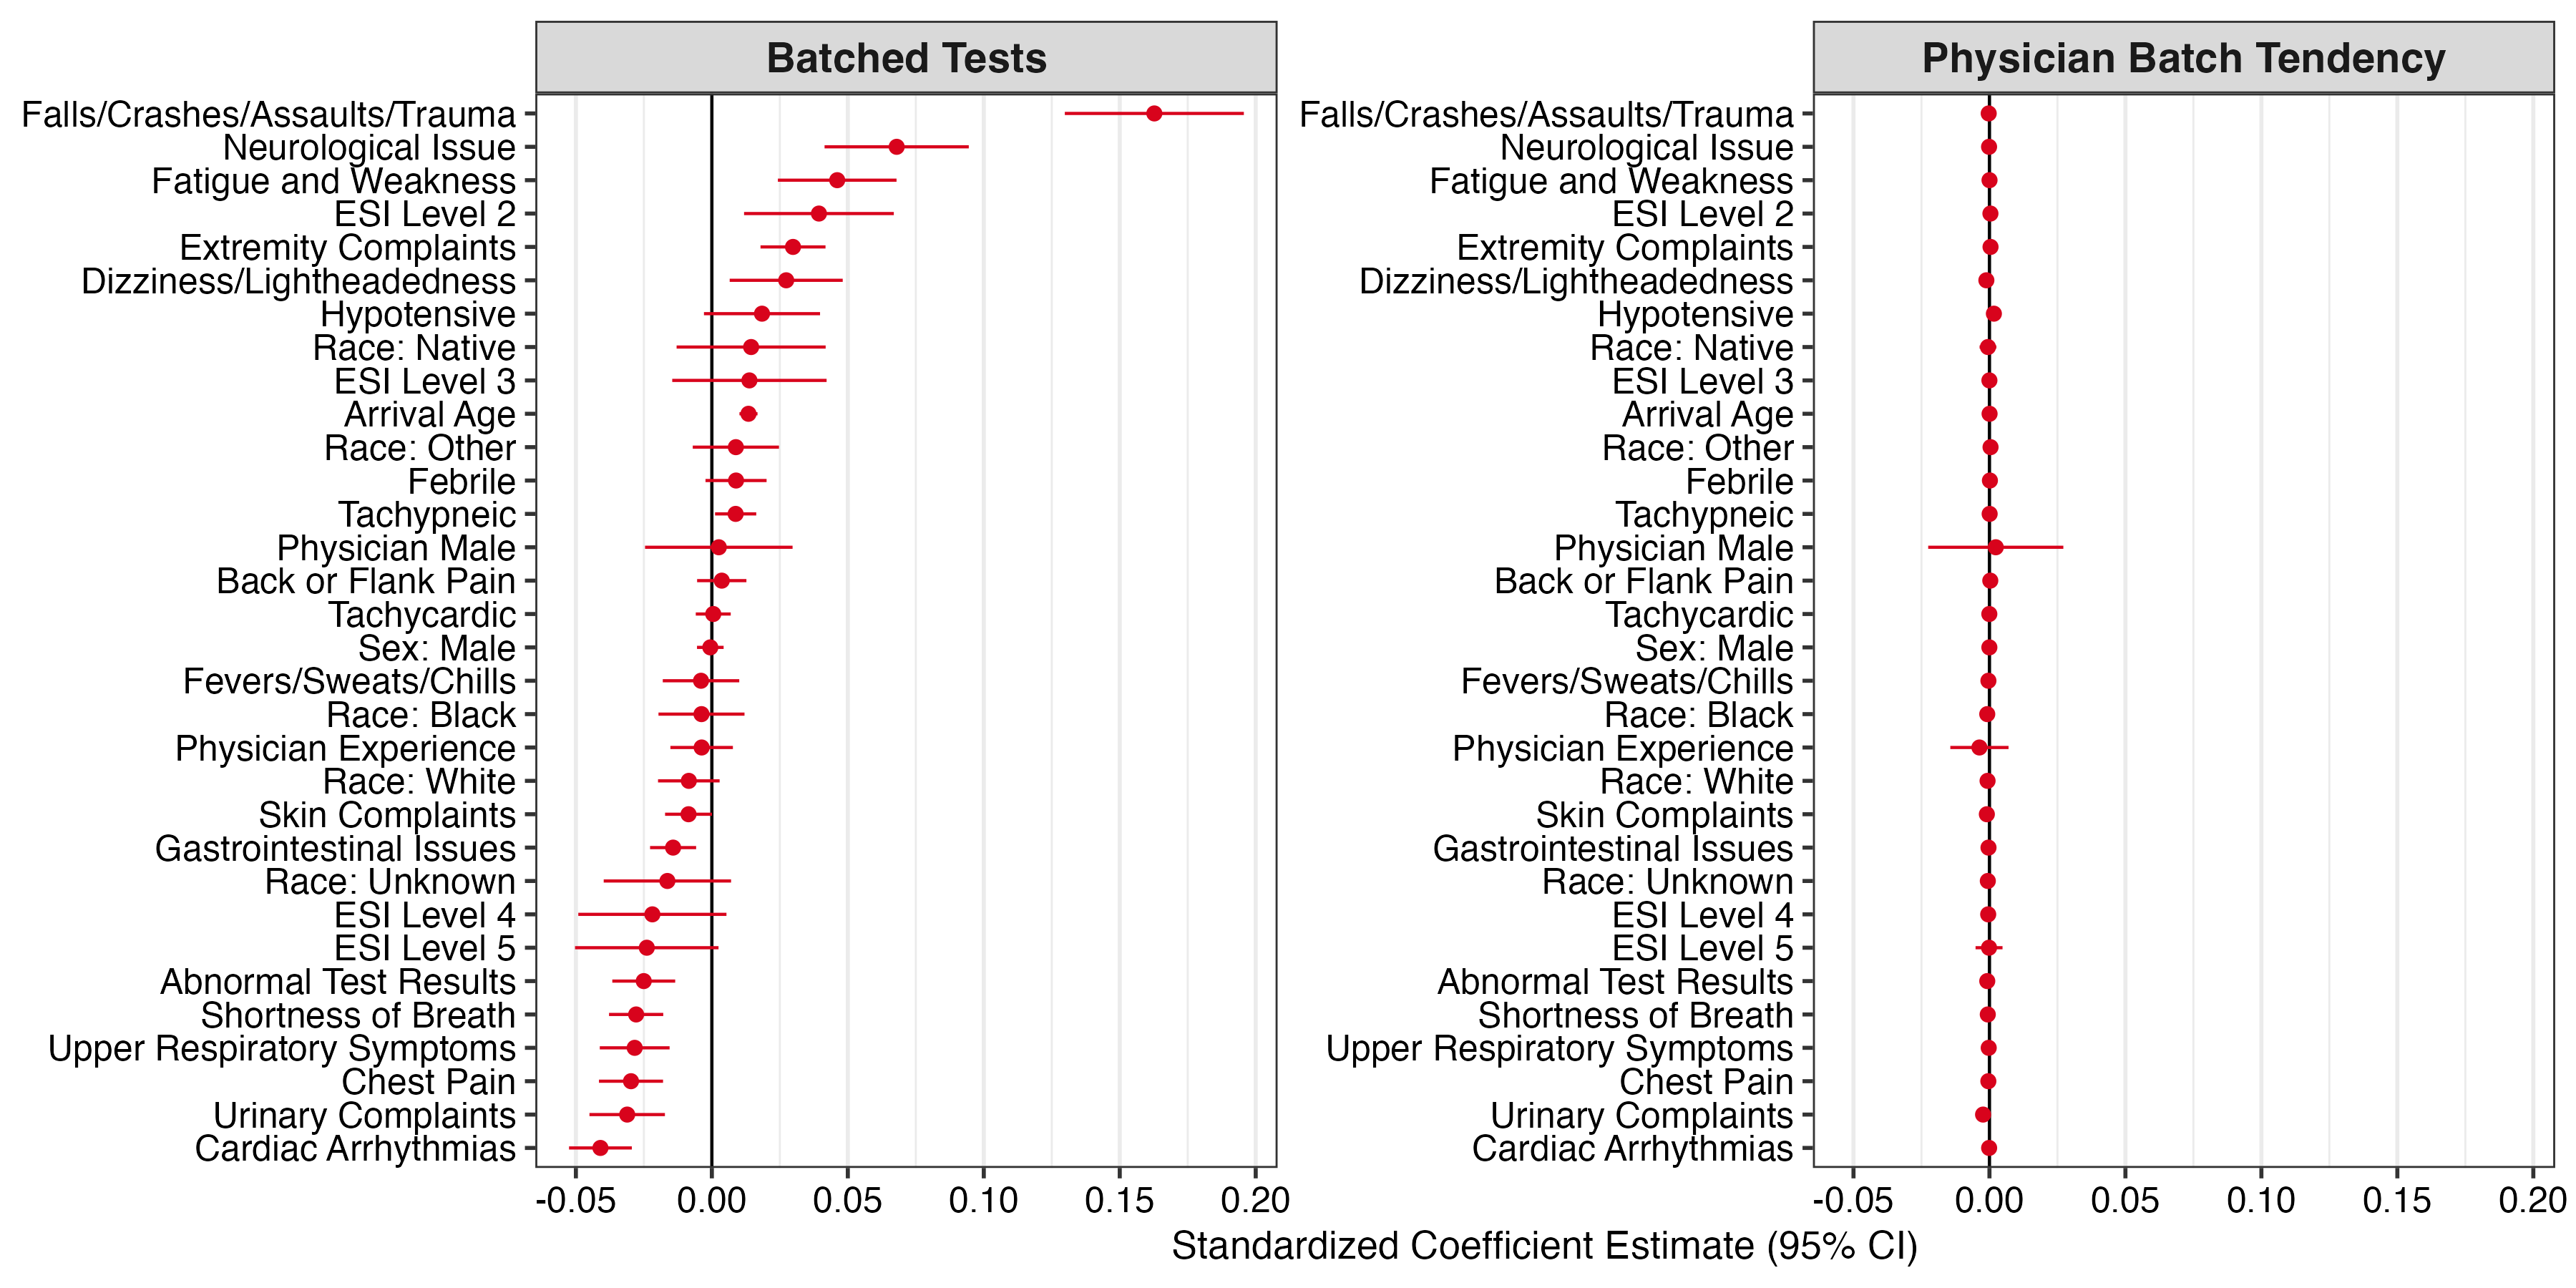
\includegraphics[width=\textwidth]{../outputs/figures/fig2_panel_batched_standardized.png}
    \begin{tablenotes}
        \small
        \item \textit{Notes:} This figure plots a test for quasi-random assignment of patients to physicians in the Mayo Clinic ED. The left panel shows how patient characteristics predict batching decisions. The right panel shows these same characteristics do not predict assignment to physicians with different batch tendencies. Residualization fixed effects include hospital-year-month, hospital-day of week-time of day. Robust standard errors are clustered at the physician level.
    \end{tablenotes}
\end{threeparttable}
\end{figure}

Together, the institutional details and empirical balance tests confirm that Mayo Clinic's rotational assignment mechanism achieves the quasi-randomization necessary for our identification strategy. This distinguishes our study from observational analyses where endogenous patient-physician matching could confound estimates of physician practice effects.

\color{black}



%%%%%%%%%%%%%%%%%%%%%%%%%%%  R1 Comment 5  %%%%%%%%%%%%%%%%%%%%%%%%%%%%%%%%%%
\begin{quote2}
\textbf{R1 Wrote (Potential impact \& writing quality):}

\noindent``The paper is well written, and studies an important question. I hope the authors find this report helpful in moving this work forward.” 
\end{quote2}

\noindent\textbf{***Response:} \textcolor{blue}{We sincerely thank the reviewer for their thorough and constructive feedback. The detailed comments have been invaluable in strengthening our analysis and clarifying our contributions. We believe the extensive revisions addressing the reviewer's concerns about variable definition, empirical strategy, and causal interpretation have substantially improved the manuscript.}


%%%%%%%%%%%%%%%%%%%%%%%%%%%%%%%%%%%%%%%%%%%%%%%%%%%%%%%%%%%%%%%%%%%%%%%%%%%%%%
% End of Reviewer 1 responses
%%%%%%%%%%%%%%%%%%%%%%%%%%%%%%%%%%%%%%%%%%%%%%%%%%%%%%%%%%%%%%%%%%%%%%%%%%%%%%

\clearpage

%%%%%%%%%%%%%%%%%%%%%%%%%%%%%%%%%%%%%%%%%%%%%%%%%%%%%%%%%%%%%%%%%%%%%%%%%%%%%%
%%  SECTION V – RESPONSES TO REVIEWER 2 COMMENTS                           %%
%%%%%%%%%%%%%%%%%%%%%%%%%%%%%%%%%%%%%%%%%%%%%%%%%%%%%%%%%%%%%%%%%%%%%%%%%%%%%%

\pagestyle{fancy}
\fancyhead{}
\fancyhead[RO,RE]{\small{Responses to Referee 2 Comments}}
\renewcommand{\headrulewidth}{0pt}

\noindent\underline{\textbf{IV. Responses to Referee 2 (R2) Comments}}

%%%%%%%%%%%%%%%%%%%%%%%%%%%  R2 Comment 1  %%%%%%%%%%%%%%%%%%%%%%%%%%%%%%%%%%


\begin{quote2}
\textbf{R2 Wrote (Research question \& contribution:):}  

\noindent``The paper’s research question is clear. The main contribution is to provide causal evidence that batch ordering of advanced imaging tests in emergency departments (EDs) — commonly assumed to be efficient — increases patient length of stay (LOS), test volume, and admission rates. EDs are under constant pressure to improve throughput, and advanced imaging is a major driver of delays, costs and overcrowding in the EDs. The paper does have the potential to make a significant and novel contribution by causally examining the impact of diagnostic batch ordering in emergency departments. While prior research has explored physician-driven variation in testing and the operational burden of imaging, this study uniquely isolates the effect of batching behavior using a quasi-randomized design.”
\end{quote2}

\noindent\textbf{Response:} \textcolor{blue}{We appreciate the reviewer's recognition of our contribution to understanding diagnostic test ordering in emergency departments. We agree that challenging the conventional wisdom about batch ordering efficiency is important given the operational pressures EDs face. The reviewer's acknowledgment that our quasi-randomized design uniquely isolates batching effects validates our empirical approach. Following the reviewer's and other referees' suggestions, we have further clarified how our findings differ from prior work on physician practice variation by specifically focusing on the timing and sequencing of test orders rather than just testing intensity.}

\begin{quote2}
\textbf{R2 Wrote (Framing):}  


\noindent``The paper frames the comparison as "batching vs. sequential", but that is not technically correct. In reality, the way the independent variable is defined, the comparison is “early batched imaging” vs. “everything else”, which includes a broad mix of clinical pathways. This muddies the interpretation: are the harms of batching due to: The batching itself? Or just differences between patients who need 2+ early tests vs. those who do not? Moreover, the sequencing is not fully explored: the study favors sequential ordering, but the authors do not actually compare different sequencing strategies or evaluate outcomes where delayed imaging causes diagnostic delays.”
\end{quote2}


\noindent\textbf{Response:} \color{blue}We thank the reviewer for this important clarification about our treatment comparison. The reviewer is absolutely correct that our empirical strategy compares ``early batched imaging" with ``everything else" rather than a pure batching versus sequential comparison. This point was raised by the other reviewers as well. We appreciate this opportunity to clarify our approach and have made substantial revisions to address this concern.

First, an essential clarification: our sample includes only encounters where at least one imaging test was ordered. The "everything else" comparison therefore comprises patients who received either (1) a single imaging test, or (2) multiple tests ordered sequentially—but not patients with zero imaging. This distinction is critical because our comparison is between different imaging strategies for patients requiring diagnostic imaging, not testing versus no testing. That said, the reviewer is correct that our counterfactual remains composite—mixing single-test and sequential multi-test encounters.

The reviewer raises a fundamental question: are the harms from batching itself or from differences between patients needing multiple early tests? This gets to the heart of causal inference in our setting. For decisions at the margin of physciain discretion, such as the one we study, the batching decision is made under uncertainty about whether additional tests will be needed. Conditioning our analysis on eventual test count would introduce post-treatment bias, as the initial ordering strategy causally affects subsequent testing decisions. Our approach preserves causal interpretation by comparing strategies at the moment of decision-making.

We have made the following changes to address your concerns which we believe have made the manuscript stronger:

\begin{enumerate}
    \item \textbf{Reframed our comparison throughout the manuscript}. We now consistently describe our comparison as ``batch ordering versus standard practice" rather than "batching versus sequencing." 
    
    \item \textbf{Clarified what we identify and why it matters}. We added text in Section 3.3 explaining:
    \begin{quote}
    ``Our two-stage least squares estimates represent the LATE of batch ordering for `compliers'---patients whose testing strategy depends on the assigned physician's practice style. This effect compares batch ordering to standard practice, which includes both sequential ordering and single tests. While this involves a composite counterfactual, it provides the policy-relevant parameter: the effect of encouraging comprehensive upfront testing versus allowing diagnostic information to guide testing decisions for patients at the margin of clinical discretion—those whose testing strategy is not dictated by clear clinical necessity but rather depends on physician practice style and judgment."
    \end{quote}
    
    \item \textbf{Added discussion of the information problem}. In Section 3.2.1, we explain why we focus on early batching:
    \begin{quote}
    ``We focus on batches that concern the first imaging tests ordered during the patient encounter because this represents the moment of maximum diagnostic uncertainty, when physicians must decide their testing strategy before clinical information unfolds. Physicians cannot know ex-ante which patients will ultimately require multiple tests, leading to instances of early batching as discretionary choice based on practice style rather than clinical necessity."
    \end{quote}

Regarding potential harms from delayed sequential testing, we find no evidence on 72-hour return, suggesting sequential approaches do not cause harmful diagnostic delays.

\item \textbf{Clarified why ``everything else" is the right comparison}. We added to Section 5.1:
\begin{quote}
    ``This comparison reflects the real choice facing ED managers: should protocols encourage comprehensive upfront testing or preserve diagnostic flexibility? Our estimates show that preserving optionality through standard practice—which allows information from initial tests to guide subsequent decisions—reduces testing intensity."
\end{quote}
\end{enumerate}

The reviewer's observation about mixed clinical pathways in our counterfactual is astute. However, this heterogeneity reflects what makes our estimate policy-relevant. ED managers cannot randomize patients to pure sequential protocols based on eventual diagnostic needs (which are unknown ex-ante). They can only influence whether physicians default to comprehensive early testing or preserve diagnostic optionality when facing uncertainty. Our LATE provides exactly this parameter.

We believe these revisions substantially improve the manuscript's clarity while maintaining scientific rigor. The comparison we identify—batch ordering versus standard practice for marginal patients—is both what we can credibly estimate given the information structure and what policymakers need to know. We are grateful to the reviewer for pushing us to clarify this important distinction, as it has led us to better articulate both the methodological foundations and practical implications of our work.

\color{black}

%%%%%%%%%%%%%%%%%%%%%%%%%%%  R2 Comment 3  %%%%%%%%%%%%%%%%%%%%%%%%%%%%%%%%%%
\begin{quote2}
\textbf{R2 Wrote (Hypotheses):}  

\noindent``As it currently stands, the study lacks a clearly articulated hypotheses section, which would help clarify the underlying mechanisms the authors expect to observe in the results. This section is typically where one would expect the authors to build a narrative around the anticipated behavioral patterns and how those behaviors are theoretically linked to the operational outcomes under study.” 
\end{quote2}

\noindent\textbf{Response:} \color{blue}We thank the reviewer for this valuable suggestion to develop formal hypotheses. The reviewer is absolutely correct that explicitly articulating our theoretical predictions strengthens the paper's contribution and clarifies the mechanisms we expect to observe.

Following this guidance, we have added Section 2.3 ``Hypothesis Development" that builds from our literature review to develop four formal hypotheses about how batch ordering affects ED operations:

\begin{quote}
\subsection*{``Hypothesis Development}

Building on the literature reviewed above, we develop formal hypotheses about how batch ordering affects ED operations. While prior work has identified the mechanisms driving batching behavior and its potential consequences, the net effects remain theoretically ambiguous. Our theoretical framework centers on the fundamental tradeoff between the perceived efficiency of parallel processing and the information value of sequential testing.

\subsubsection*{Information Value and Test Volume}

The decision to batch or sequence tests fundamentally involves whether to preserve the option value of information. Sequential testing allows each test result to inform subsequent decisions, potentially eliminating unnecessary tests. When physicians batch tests upfront, they commit to a diagnostic pathway before information unfolds, forfeiting this option value.

Physicians under high workloads face cognitive strain from task switching and may batch tests to defer complex diagnostic reasoning \cite{kc2013does, skaugset2016can}. However, this cognitive convenience comes at a cost. Without the filtering mechanism of sequential information revelation, physicians must rely solely on their initial assessment. \cite{lam2020why} identify this as a key driver of overtesting---when facing diagnostic uncertainty, physicians order comprehensive test batteries rather than allowing initial results to guide subsequent testing. Given the documented variation in physician testing intensity \cite{hodgson2018are}, with some physicians ordering twice as many tests as their peers, batching likely amplifies these tendencies by removing the natural stopping points that sequential results provide. Therefore:

\begin{quote}
\small
\textit{\textbf{Hypothesis 1.} Batch ordering will increase the total number of imaging tests performed compared to standard practice due to the loss of information value from initial test results.}
\end{quote}

\subsubsection*{Processing Time and Operational Flow}

While batching strategies reduce setup times in manufacturing \cite{Fowler2022}, the ED imaging context presents unique operational constraints as noted in our review. Different imaging modalities require separate equipment and cannot be performed simultaneously \cite{Jessome2020}. This creates a fundamental bottleneck where batched orders must still be executed sequentially, but now with a larger committed workload that cannot be adjusted based on emerging information.

Moreover, the cognitive load literature suggests that processing multiple test results simultaneously increases decision complexity \cite{kc2013does}. When physicians receive multiple results at once rather than sequentially, they must integrate more information simultaneously, potentially lengthening the diagnostic reasoning process. This "information overload" effect, combined with the additional tests ordered as predicted in H1, suggests that batching may paradoxically increase rather than decrease processing times:

\begin{quote}
\small
\textit{\textbf{Hypothesis 2.} Batch ordering will increase patient length of stay and time to disposition compared to standard practice, as the operational constraints of imaging and increased test volume outweigh any potential benefits of parallel processing.}
\end{quote}

\subsubsection*{Clinical Decision-Making and Disposition}

The medical literature recognizes ``diagnostic momentum"---where abnormal findings, even if clinically insignificant, drive further workup and more conservative clinical decisions \cite{coen2022clinical; featherston2020decision}. When physicians batch order and receive multiple results simultaneously, they encounter more opportunities for incidental findings that may influence disposition decisions \cite{lumbreras2010incidental, berlin2011incidentaloma}. As our review noted, physicians facing uncertainty and potential legal consequences may opt for more conservative disposition decisions \cite{rao2012overuse, lam2020why}. The simultaneous arrival of multiple test results, particularly with incidental findings, may trigger defensive medicine behaviors:

\begin{quote}
\small
\textit{\textbf{Hypothesis 3.} Batch ordering will increase hospital admission rates through increased diagnostic intensity and the influence of incidental findings on clinical decision-making.}
\end{quote}

\subsubsection*{Contextual Moderators}

The literature on physician behavior under capacity constraints consistently shows that resource scarcity forces more selective decision-making \citep{kuntz2014stress, kc2009impact}. When EDs face severe overcrowding, the operational pressures documented in our review intensify. Under these conditions, physicians may reserve batching for cases where it is clinically essential rather than convenient:

\begin{quote}
\small
\textit{\textbf{Hypothesis 4.} The effects of batch ordering on LOS and test volume will be attenuated under conditions of major ED overcapacity, as physicians become more selective in their batching decisions.}
\end{quote}

These hypotheses provide testable predictions that we examine using our quasi-experimental design. By leveraging variation in physician batching tendency under random patient assignment, we can identify whether these theoretical mechanisms manifest in actual ED operations."
\end{quote}

This new section provides the theoretical foundation that motivates our empirical specifications and helps readers understand which mechanisms we test. We are grateful to the reviewer for this suggestion, which has substantially strengthened the manuscript's theoretical contribution.

\color{black}


%%%%%%%%%%%%%%%%%%%%%%%%%%%  R2 Comment 4  %%%%%%%%%%%%%%%%%%%%%%%%%%%%%%%%%%
\begin{quote2}
\textbf{R2 Wrote (Shift‑of‑testing to other settings):}  
``While the study finds that batch ordering increases imaging in the ED as well as inpatient admissions, it does not evaluate whether this reflects actual overuse or a shift in imaging from the inpatient setting to the ED. In other words, it is unclear whether batching increases unnecessary testing or simply frontloads diagnostics."

\end{quote2}

\noindent\textbf{Response:} \color{blue}We thank the reviewer for this important distinction between overuse and frontloading of diagnostics. The reviewer is correct that we cannot definitively determine whether the additional imaging represents unnecessary testing or simply shifts testing from inpatient to ED settings. This is an important limitation of our study.

However, interpreting our findings purely as frontloading faces a conceptual challenge. Frontloading would imply batched patients receive ED tests that would have been ordered during a predetermined hospitalization. Yet admission itself is a downstream consequence of the testing strategy in our data—we find that batching increases admission probability through increases in imaging tests performed. This suggests at least some proportion of the additional tests are driving new admission decisions rather than frontloading diagnostics for patients who would have been admitted regardless of their ED imaging results. That is, the tests themselves are creating admissions, not being ordered because admission was already determined.

That said, we acknowledge multiple causal pathways may operate simultaneously. Some batched patients may receive tests that genuinely reveal admission-worthy conditions that would have been discovered later. Others may be admitted defensively due to incidental findings from comprehensive imaging that would not have been pursued under sequential testing. Without linked inpatient imaging records, we cannot empirically separate these mechanisms.

We have been careful throughout the manuscript to avoid characterizing the additional tests as "waste" or "overuse," as our LATE identifies effects for marginal patients whose testing decisions vary by physician preference—these tests may have clinical value regardless of timing. However, even if batching represents frontloading rather than overuse, it has operational consequences worth noting. Based on discussions with our physician coauthors at both study sites: ED imaging resources are typically more constrained than inpatient resources, frontloading increases ED congestion and delays care for other ED patients, and inpatient teams often prefer directing their own diagnostic approach based on evolving clinical information.

We have added discussion of this limitation in Section 5.3:

\begin{quote}
"We cannot determine the extent to which the additional imaging from batching represents unnecessary testing or frontloading of diagnostics that would eventually occur in the inpatient setting. However, interpreting our findings purely as frontloading is complicated by the fact that admission itself is affected by batching—we observe a 39 percentage point increase in admission probability, suggesting the tests themselves influence disposition decisions. Multiple mechanisms may operate: some additional tests may reveal genuine admission-worthy conditions, while others may trigger defensive admissions through incidental findings. Distinguishing between these pathways would require linked ED-inpatient imaging data to examine whether batched patients receive correspondingly fewer tests after admission. This remains an important direction for future research."
\end{quote}

We appreciate the reviewer highlighting this distinction, as it has led us to be more precise about the causal pathways our estimates capture and the important questions that remain for future research.

\color{black}

%%%%%%%%%%%%%%%%%%%%%%%%%%%  R2 Comment 5  %%%%%%%%%%%%%%%%%%%%%%%%%%%%%%%%%%
\begin{quote2}
\textbf{R2 Wrote (Request for cost‑benefit analysis):} 

\noindent``Relatedly, what would help is a cost-benefit analysis -- given the
findings about overuse, it is surprising the paper does not estimate financial impact or
imaging cost burdens. Do the authors have any data they could use to conduct such an
analysis?” 
\end{quote2}

\noindent\textbf{Response:} \textcolor{blue}{[Your response here]}

%%%%%%%%%%%%%%%%%%%%%%%%%%%  R2 Comment 6  %%%%%%%%%%%%%%%%%%%%%%%%%%%%%%%%%%
\begin{quote2}
\textbf{R2 Wrote (Batch timing and its relation to LOS):}

\noindent``Batch timing is unclear to me. Specifically, Length of Stay (LOS) is used as a primary outcome. Batching, defined as imaging orders within the first 5 minutes of encounter, is treated as a treatment applied at the beginning of the visit. But in real ED workflows, the decision to batch may itself be a function of how the patient’s case has unfolded up to that point. For example, if the diagnosis is taking longer, or prior tests have not resolved the issue, or if the physician senses the patient may be admitted soon, then the physician might batch several tests later in the encounter in order to “wrap things up” and avoid delays — i.e., batching becomes a consequence of extended LOS, not just a cause. The 5-minute window may not capture the delayed batching; e.g., if initial results come back inconclusive or the patient’s condition worsens. Thus, the batching variable may be misclassified, and later batches that react to prolonged stays are excluded from the analysis. Even when orders are placed early, test results often take time to return. That delay — especially from CTs or MRIs — inflates LOS. Therefore, the measured LOS may not be a clean posttreatment outcome, but instead partially determined by the batching process itself. This risks simultaneity bias, where cause and effect are entangled in time. The issue is less severe if the paper really only claims to understand something about initial batching decisions, but I am not sure the authors have made those distinctions clear enough.” 
\end{quote2}

\noindent\textbf{Response:} \color{blue}We thank the reviewer for this insightful observation about the temporal relationship between batching and LOS. This comment has led us to substantially clarify throughout the manuscript that our study specifically examines discretionary early batching decisions—those made at the beginning of encounters in the very first set of tests ordered under diagnostic uncertainty. These are precisely the decisions where physician practice style dominates clinical necessity, representing the margin where ED protocols, training interventions, and decision support systems can meaningfully influence practice. Later adaptive batching in response to case complexity represents clinical judgment that managerial policies cannot and should not constrain.

\textbf{Why early batching is the relevant parameter:} The reviewer correctly notes that physicians might batch tests later to ``wrap things up." This adaptive behavior is fundamentally different from the discretionary decision to order comprehensive imaging upfront. Our instrumental variable (physician batch tendency) specifically captures variation in early ordering propensity—identifying physicians who habitually commit to comprehensive imaging before information unfolds versus those who preserve diagnostic flexibility.

Empirically, we verify that ``late batching"—cases where a single test is followed by a batch—is rare, occurring in only 189 encounters (1.91\% of multi-test encounters). To verify this classification does not impact our results, we re-estimated all models treating such cases as batched (Appendix Table X.X). The results are virtually identical, confirming our classification is appropriate.

\textbf{Clarifications made throughout the manuscript:} Following the reviewer's observation, we have revised our framing to emphasize that our parameter of interest is the effect of discretionary batching versus standard practice:

\begin{enumerate}
\item \textbf{Abstract:} Now specifies "discretionary batching decisions made at encounter initiation"

\item \textbf{Section 1.2:} Clarifies that our LATE identifies "the effect of discretionary batching for patients whose testing strategy depends on physician practice style rather than clinical necessity"

\item \textbf{Section 3.2.1:} Extensively revised to clarify our focus:
\begin{quote}
"We focus on batches that concern the first imaging tests ordered during the patient encounter because this represents the moment of maximum diagnostic uncertainty when physicians must decide their testing strategy before clinical information unfolds. Physicians cannot know ex-ante which patients will ultimately require multiple tests, making early batching a discretionary choice based on practice style rather than clinical necessity."
\end{quote}
\end{enumerate}

\textbf{LOS as outcome and simultaneity bias:} The reviewer raises an important concern about whether LOS can serve as a clean post-treatment outcome given that test completion times mechanically contribute to its measurement. We acknowledge this concern but emphasize that this relationship is not a confounder—it is precisely the causal pathway our study seeks to identify.

The reviewer asks whether this creates ``simultaneity bias, where cause and effect are entangled in time." This would be a concern if batching and LOS were simultaneously determined by some third factor, or if LOS caused batching. However, our design addresses this: we focus on early batching decisions (first tests ordered of the encounter), and our instrument (physician batch tendency) is predetermined before the patient encounter begins. The temporal ordering is clear: physician tendency $\rightarrow$ batching decision $\rightarrow$ test ordering $\rightarrow$ test completion $\rightarrow$ LOS. The mechanical relationship between test completion and LOS represents the causal pathway through which early batching operates, not simultaneity bias.

Our treatment is the decision to batch, and LOS captures the total consequences of that decision. When physicians choose to batch tests upfront, they set in motion a cascade of operational consequences: patients wait for multiple tests to complete, radiologists must interpret multiple images, physicians must cognitively process all results simultaneously, and clinical decisions must integrate potentially conflicting or incidental findings. These are the mediating mechanisms through which early batching decisions affect patient flow.

Our mediation analysis (Section 4.3) formally decomposes these pathways, revealing that increased test volume accounts for the majority of the LOS effect (indirect effect = 0.207, $p < 0.001$). This confirms that the ``mechanical" component the reviewer identifies—waiting for additional tests—is indeed a key mechanism resulting from the discretionary early batching decision.

Furthermore, to separate clinical decision-making time from test completion time, we examine "time to disposition"—the duration until physicians make admission/discharge decisions, excluding post-decision boarding. The persistence of large effects (123\% increase) demonstrates that early batching affects not just mechanical waiting but also clinical processing efficiency. Even when excluding post-disposition time (where no testing occurs), the early discretionary batching decision substantially delays clinical decision-making.

We appreciate the reviewer's careful attention to these temporal dynamics, which has prompted us to more clearly articulate that our study evaluates the full operational consequences of discretionary early batching decisions—precisely the parameter ED managers need to understand when considering protocols to influence physician ordering behavior.
\color{black}


%%%%%%%%%%%%%%%%%%%%%%%%%%%  R2 Comment 7  %%%%%%%%%%%%%%%%%%%%%%%%%%%%%%%%%%
\begin{quote2}
\textbf{R2 Wrote (Definition of batching):}  
``The definition of batching is also narrowly defined to be 2+ tests ordered within the 5 first minutes. The study equates batch ordering with guaranteed test completion and additive imaging volume. However, in practice, test results may return asynchronously, and physicians may update their diagnostic plans based on early results—even for batched orders. For example, even if the physicians initially batch ordered the tests, they could cancel some of these as they review the results. The paper would benefit from clarifying how often batched tests were actually completed and whether sequential result review modified downstream test execution. Without this, the causal link between batch ordering and increased imaging intensity may be overstated.” 
\end{quote2}

\noindent\textbf{Response:} \color{blue}
We thank the reviewer for this important clarification question. Our outcome measures count imaging tests actually performed, not merely ordered. This critical distinction strengthens our causal interpretation: the 1.4 additional tests per marginally batched patient represent completed imaging studies that consumed resources and time, not provisional orders subsequently cancelled.

Based on consultation with our physician coauthor at Mayo Clinic, test cancellations after batch ordering face substantial operational barriers. Once the radiology department acknowledges an order, cancellation requires physicians to physically call and request the department to "push back" the imaging order. Furthermore, radiology departments often coordinate between modalities (e.g., CT and ultrasound) so patients move directly from one scanner to another. With radiologist read times averaging 60 minutes, patients typically complete all batched imaging before initial results become available for physician review. While cancellations occasionally occur (e.g., a CT scan revealing appendicitis leading to a cancelled pelvic ultrasound), the operational friction makes these exceptions rather than the standard practice.

Importantly, even if some batched orders were cancelled, this would render our estimates conservative. Cancelled tests still consume operational resources—patients are queued, transported, and prepared for imaging that ultimately does not occur. These inefficiencies from cancelled tests would represent an additional operational burden beyond what our completed test counts capture. Thus, our measure of performed tests likely represents a lower bound on the actual operational impact of batching behavior.

\textbf{Manuscript changes made throughout:}

We have clarified the distinction between ordered and performed tests in multiple sections:

Section 3.2.2 (Dependent Variables): 
\begin{quote}
``Beyond time-based metrics, we examine resource utilization through the number of distinct imaging tests performed during each ED encounter. This count variable helps us understand how batch ordering practices influence the diagnostic workload."
\end{quote}

Section 4.2 (Results): Added clarification: 
\begin{quote}
``Discretionary batching also leads to more intensive diagnostic testing. Specifically, the marginal batched patient receives 1.4 more distinct imaging tests (completed studies with documented results), representing a 105\% increase from the mean for sequentially tested patients."
\end{quote}

Table 4: Added footnote: 
\begin{quote}
``Test counts represent performed imaging studies with documented results, not ordered tests. The persistence of increased test volume under batching suggests cancellations do not substantially offset the effect."
\end{quote}

Section 5.3 (Limitations): Added: 
\begin{quote}
``Our data contains imaging tests that were both ordered and performed. We cannot observe tests that were ordered but subsequently cancelled before completion. However, test cancellation after ordering requires substantial coordination—physicians must call the radiology department to remove patients from imaging queues. This operational friction makes cancellations rare. Moreover, cancelled tests introduce their own inefficiencies: patients experience delays from queuing and preparation, while ED resources are allocated to coordinate cancellations. To the extent that batched orders are more likely to include tests that are ultimately cancelled, our estimates of performed tests would understate the true operational burden of batching behavior."
\end{quote}

These clarifications ensure that readers understand our analysis captures actual resource utilization and that potential cancellations would, if anything, strengthen rather than weaken our conclusions about the operational burden of batching.

\color{black}

%%%%%%%%%%%%%%%%%%%%%%%%%%%  R2 Comment 8  %%%%%%%%%%%%%%%%%%%%%%%%%%%%%%%%%%
\begin{quote2}
\textbf{R2 Wrote (Role of laboratory results):}  

\noindent``While the study restricts its scope to imaging due to its operational constraints, it does not address the interplay and potential dependencies between imaging and other diagnostic inputs—particularly lab results. One can imagine that in practice, lab results often arrive earlier and may prompt physicians to reassess imaging decisions, even when tests are initially batched. Could this potentially overstate the causal impact of batching on downstream outcomes?” 
\end{quote2}

\noindent\textbf{Response:} \color{blue}
We thank the reviewer for raising this important concern about whether earlier-arriving lab results might affect our estimates of batching's causal impact. This insightful observation prompted us to empirically examine the potential interplay between laboratory and imaging pathways, which has strengthened our analysis.

The reviewer correctly notes that lab results often arrive before imaging results (typically 30-60 minutes for basic labs versus 90-165 minutes for imaging). Based on consultation with our physician co-author at the Mayo Clinic, normal lab results typically do not lead to imaging cancellation. Cancellation occurs only in rare, extreme cases: when labs provide a definitive diagnosis (e.g., severe anemia fully explaining dyspnea, thereby eliminating the need for a chest CT) or when results indicate instability precluding imaging (e.g., severe hyperkalemia requiring immediate dialysis). More commonly, abnormal lab results might modify the imaging type—for instance, switching from contrast to non-contrast CT for acute kidney injury—but do not eliminate the need for imaging. Importantly, even these modifications require physicians to call the radiology department, creating a significant workflow barrier that discourages treating batch orders as provisional.

Given these operational realities, imaging cancellations based on lab results are rare.  Our outcome measures count performed tests, not ordered tests, so any cancellations  that do occur would make our estimates conservative—we would be understating the  initial commitment to imaging that batching represents. The fact that we observe 1.4  additional performed imaging tests per marginally batched patient demonstrates that  batched imaging pathways, once initiated, proceed to completion despite the theoretical possibility of modification based on lab results.

To empirically test whether lab results moderate our batching effects, we examined specifications progressively adding controls. Following concerns from Reviewers 1 and 3 about potential exclusion restriction violations, we first added physician characteristics to ensure our instrument captures batching behavior specifically rather than other physician attributes. We then added lab ordering to test for lab-imaging interactions:

\begin{table}[h]
\centering
\caption*{Robustness of Batching Effects to Additional Controls}
\begin{threeparttable}
\begin{tabular}{lccc}
\toprule
& Baseline & + Physician & + Lab \\
& Controls & Characteristics & Ordered \\
& (1) & (2) & (3) \\
\midrule
\multicolumn{4}{l}{\textit{Panel A. Primary Outcomes}} \\[0.5em]
Log time to disposition & $0.804^{*}$ & $0.822^{*}$ & $0.771^{.}$ \\
& (0.349) & (0.374) & (0.395) \\[0.5em]
Log LOS & $0.837^{*}$ & $0.854^{*}$ & $0.673^{*}$ \\
& (0.299) & (0.328) & (0.323) \\[0.5em]
Number of imaging tests & $1.414^{***}$ & $1.373^{***}$ & $1.263^{***}$ \\
& (0.220) & (0.207) & (0.197) \\[0.5em]
72hr return with admission & -0.012 & -0.012 & -0.015 \\
& (0.018) & (0.020) & (0.023) \\[0.5em]
\midrule
Controls included: \\
Time FE & Yes & Yes & Yes \\
Patient characteristics & Yes & Yes & Yes \\
Physician characteristics & No & Yes & Yes \\
Lab ordered indicator & No & No & Yes \\
\midrule
Observations & 11,404 & 11,404 & 11,404 \\
\bottomrule
\end{tabular}
\begin{tablenotes}
\footnotesize
\item \textit{Notes:} All columns show 2SLS estimates. Column 1 reproduces our main specification from Table 4. Column 2 adds physician characteristics (experience, gender) to address exclusion restriction concerns. Column 3 further adds an indicator for whether labs were ordered. While some attenuation occurs with lab controls, all specifications show large, economically meaningful effects.
\item $^{.} p < 0.1$, $^{*} p < 0.05$, $^{***} p < 0.001$.
\end{tablenotes}
\end{threeparttable}
\end{table}

We observe modest attenuation when controlling for laboratory ordering, with the log time to disposition effect decreasing from 0.822 to 0.771 and losing some statistical precision. This attenuation suggests that physicians who batch imaging tests also tend to order laboratory tests, reflecting a broader pattern of comprehensive diagnostic ordering. When we control for this general diagnostic intensity through the lab indicator, we isolate the effect of imaging batching more precisely. Importantly, even after accounting for concurrent lab ordering, all specifications show large, economically meaningful effects on processing times and imaging volume. The persistence of these substantial effects demonstrates that discretionary imaging batching creates operational burdens beyond what can be explained by general diagnostic thoroughness, confirming that batched imaging pathways proceed independently once initiated due to operational momentum and workflow barriers to modification.

\textbf{Manuscript changes:}

\textit{Section 4.8 (Robustness):} Added Table A.Z with the above specifications and 
discussion addressing this concern:
\begin{quote}
``To address concerns about lab-imaging interactions, we examined whether controlling for laboratory ordering affects our estimates of discretionary batching (Table A.Z). The modest attenuation when adding lab controls (e.g., log time to disposition: 0.822 to 0.771) indicates that some portion of our estimated batching effect reflects correlation with general diagnostic intensity—physicians who batch imaging also tend to order more laboratory tests. By controlling for lab ordering, we isolate the imaging-specific component of the batching effect. Importantly, even after decoupling this correlation, we find large, persistent impacts in processing times and imaging volume. This demonstrates that discretionary imaging batching creates substantial operational burdens distinct from broader diagnostic thoroughness. Clinical evidence supports this independence: normal lab results rarely lead to imaging cancellation, as modifications require calling radiology departments—a significant workflow barrier. The persistence of large effects after controlling for laboratory utilization confirms that discretionary batching commits patients to imaging pathways that proceed independently once initiated."
\end{quote}

We appreciate the reviewer highlighting this potential concern, as addressing it demonstrates the robustness of our findings and clarifies that discretionary batching creates operational commitments that persist despite the theoretical possibility of lab-based modifications.

\color{black}



%%%%%%%%%%%%%%%%%%%%%%%%%%%  R2 Comment 9  %%%%%%%%%%%%%%%%%%%%%%%%%%%%%%%%%%
\begin{quote2}
\textbf{R2 Wrote (Limited scope of patient conditions):}  
 
\noindent``The study excludes many complaints where imaging is rarely ordered or batching is infeasible (e.g., dermatologic issues, urinary complaints). The results may not apply to low-acuity patient populations or fast-track EDs. Therefore, the study is more narrowly defined.” 
\end{quote2}

\noindent\textbf{Response:} \color{blue}We thank the reviewer for highlighting the focused nature of our sample. The reviewer is correct that we exclude complaints where imaging is rarely ordered or batching is uncommon (occurring less than 5\% of the time). This exclusion was necessary for both statistical and substantive reasons.

Statistically, our instrumental variables approach requires sufficient variation in batching behavior to identify effects. Including complaints where batching rarely occurs time would create weak instrument problems and yield unreliable estimates. For these rarely batched complaints, physicians have effectively determined that batching is clinically inappropriate—there is no discretionary decision to be made.

Substantively, the random assignment of patients to physicians at Mayo Clinic allows us to restrict our sample to complaints where batching is a relevant operational decision without introducing selection bias. This focused approach provides clear, actionable insights for specific clinical scenarios—trauma, neurological complaints, abdominal pain—where batching decisions are actively debated among emergency physicians and meaningfully impact ED operations. These complaints represent approximately 25\% of the ED volume but account for 41\% of imaging resource utilization in our data, underscoring their operational significance.

We agree that this narrows the scope of our study. However, this focus ensures our estimates are both statistically identified and operationally relevant for the clinical contexts where batching represents a genuine debated practice choice. We have added text to the limitations section explicitly acknowledging this scope:

\begin{quote}
``Our findings apply to moderate-to-high acuity patients with complaints commonly requiring multiple imaging studies. The effects of batching in low-acuity or fast-track settings, where imaging is less common, remain unexplored."
\end{quote}


\color{black}

%%%%%%%%%%%%%%%%%%%%%%%%%%%  R2 Comment 10  %%%%%%%%%%%%%%%%%%%%%%%%%%%%%%%%%
\begin{quote2}
\textbf{R2 Wrote (Physician‑only ordering \& staffing mix):}  

\noindent``At Mayo, only emergency physicians (EPs) order imaging,
which is not standard in many EDs (where nurse practitioners, physician assistants, or
residents contribute). Does this limit the generalizability to other care settings? How
does this difference manifest itself particularly in EDs with significant staffing by parttime
or mid-level providers?” 
\end{quote2}

\noindent\textbf{Response:} \color{blue}We appreciate the reviewer raising this important point about staffing differences across EDs. The reviewer is correct that Mayo Clinic's physician-only ordering policy differs from many EDs, where nurse practitioners, physician assistants, and residents participate in ordering decisions.

However, our replication at MGH addresses this concern of generalizability directly. MGH employs a mixed staffing model where mid-level providers participate under attending supervision—more representative of typical US emergency departments. As shown in Table 7, the effects at MGH (a 44.3\% increase in LOS and 1.8 additional tests) are directionally similar and statistically indistinguishable from those at Mayo, demonstrating that the batching phenomenon persists across different staffing configurations.

Mayo's physician-only setting provides methodological advantages for causal identification by eliminating potential confounding from provider-type variation (e.g., systematic differences in ordering patterns between nurse practitioners and attending physicians) and ensuring all decisions reflect experienced clinical judgment. The random assignment mechanism is also simpler because patients cannot be triaged to different provider types based on acuity or complaint. The consistency of results at MGH—despite its more complex staffing environment—validates that batching effects persist when mid-level providers participate in care delivery.

Our physician co-authors at both sites confirm that, while ordering processes differ, the fundamental trade-offs of batching versus sequential testing remain similar across settings. That said, we acknowledge that EDs with predominantly mid-level staffing may face additional dynamics not fully captured in our analysis, such as supervision requirements or handoff patterns that could interact with batching decisions. We have added text to Section 4.6:

\begin{quote}
``While Mayo Clinic's physician-only ordering differs from many EDs, this provides cleaner identification of batching effects. Our replication at MGH—with its mixed staffing model including mid-level providers—demonstrates that these effects persist across different provider configurations, though the specific dynamics in EDs with predominantly mid-level staffing warrant future research."
\end{quote}
\color{black}


%%%%%%%%%%%%%%%%%%%%%%%%%%%  R2 Comment 11  %%%%%%%%%%%%%%%%%%%%%%%%%%%%%%%%%
\begin{quote2}
\textbf{R2 Wrote (Sensitivity of results – Table 4):}  

\noindent``I would urge the authors to discuss the difference in results between column 4 and 5 of Table 4, specifically with regards to sensitivity to influential controls, since the results before and after adding controls differ significantly."
\end{quote2}

\noindent\textbf{Response:} \color{blue}We thank the reviewer for drawing attention to the comparison between columns 4 and 5 in Table 4. Upon careful examination, we find that adding baseline controls (column 5) demonstrates the robustness of our results rather than problematic sensitivity to influential controls.

Specifically, the point estimates remain consistently large and positive across specifications:
\begin{itemize}
    \item Log time to disposition: 0.627 (SE: 0.460) → 0.804 (SE: 0.349)
    \item Log LOS: 0.690 (SE: 0.299) → 0.837 (SE: 0.299)  
    \item Number of imaging tests: 1.395 (SE: 0.220) → 1.414 (SE: 0.220)
    \item 72hr return with admission: -0.015 → -0.012 (both near zero and insignificant)
\end{itemize}

In each case, point estimates remain economically significant with confidence intervals that substantially overlap. The primary change is an improvement in statistical precision. Adding controls reduces standard errors by accounting for patient heterogeneity (including age, vital signs, and severity of chief complaint) and temporal variation, allowing us to estimate the batching effect more precisely. For instance, the standard error for log time to disposition decreases from 0.460 to 0.349, moving the estimate from marginally significant to clearly significant at conventional levels.

The slightly larger changes in time-based outcomes (a 20-28\% increase in point estimates) compared to test counts (a 1\% change) likely reflect that time outcomes have more residual variance that controls can explain. Patient characteristics, such as age and vital signs, directly affect how long processing takes, but have less impact on the discrete decision of how many imaging modalities to order. This differential sensitivity is expected, given the nature of the outcomes, and does not change our substantive conclusions—batching increases both processing time and test volume across all specifications.

This pattern—stable direction and magnitude with improved precision—is precisely what we expect when adding relevant covariates that explain outcome variation but are orthogonal to our instrument (due to random assignment). The controls are not "influential" in the sense of dramatically changing our estimates; instead, they reduce residual variance and sharpen our ability to detect the actual effect.

We have added a footnote to Table 4 clarifying this interpretation: ``The consistency of point estimates between columns 4 and 5 demonstrates robustness, while the improvement in precision for time-based outcomes reflects that patient characteristics explain substantial residual variance in processing times."
\color{black}

%%%%%%%%%%%%%%%%%%%%%%%%%%%  R2 Comment 12  %%%%%%%%%%%%%%%%%%%%%%%%%%%%%%%%%
\begin{quote2}
\textbf{R2 Wrote (Table 1 labeling issue):}  

\noindent``In Table 1, the independent variable and dependent variable seem reversed.” 
\end{quote2}

\noindent\textbf{***Response:} \textcolor{blue}{We thank the reviewer for catching this labeling error. We have corrected the table to properly display ``Batched" as the dependent variable and ``Batch Tendency" as the independent variable. The table now clearly shows the first-stage relationship where physician batch tendency predicts the probability of batching for a given patient encounter. We apologize for any confusion this may have caused.}

%%%%%%%%%%%%%%%%%%%%%%%%%%%  R2 Comment 13  %%%%%%%%%%%%%%%%%%%%%%%%%%%%%%%%%
\begin{quote2}
\textbf{R2 Wrote (Potential impact \& writing):}  

\noindent``The insights are policy-relevant, as they directly inform how EDs might design decision support
tools, diagnostic protocols, or physician feedback systems to reduce overuse and streamline
care. While the methodological innovation (a quasi-experimental IV strategy using random
physician assignment) may not be groundbreaking in design, its application to clinical
operations and diagnostic behavior is well-executed, adding credibility and potential for
translation.” 

\end{quote2}

\noindent\textbf{***Response:} \textcolor{blue}{We thank the reviewer for this encouraging assessment of our work's policy relevance and execution. We agree that the key contribution lies not in methodological innovation per se, but in applying rigorous causal inference methods to an important operational decision in emergency medicine that has long been debated. We are grateful that the reviewer sees the potential for our findings to inform practical interventions such as decision support tools and physician feedback systems. In response to this and other reviewers' suggestions, we have strengthened the policy implications section to provide more concrete guidance for ED managers considering interventions to optimize diagnostic test ordering practices.}


%%%%%%%%%%%%%%%%%%%%%%%%%%%%%%%%%%%%%%%%%%%%%%%%%%%%%%%%%%%%%%%%%%%%%%%%%%%%%%
% End of Reviewer 2 responses
%%%%%%%%%%%%%%%%%%%%%%%%%%%%%%%%%%%%%%%%%%%%%%%%%%%%%%%%%%%%%%%%%%%%%%%%%%%%%%
\clearpage




\pagestyle{fancy}
\fancyhead{}
\fancyhead[RO,RE]{\small{Responses to Referee 3 Comments}}
\renewcommand{\headrulewidth}{0pt}

\noindent\underline{\textbf{V. Responses to Referee 3 (R3) Comments}}

%%%%%%%%%%%%%%%%%%%%%%%%%%%  R3 Comment 1  %%%%%%%%%%%%%%%%%%%%%%%%%%%%%%%%%%


\begin{quote2}
\textbf{R3 Wrote (Research question \& contribution:):}  

\noindent``Given the growing concern about overdiagnosis in general and its potential role in exacerbating ED overcrowding, I find the research question of this paper highly relevant to emergency medicine management. Due to the individualistic nature of decision-making in EDs, emergency physicians are often perceived as “cowboy doctors.” While it may be challenging to implement strict guidelines for test-ordering behaviors in such a dynamic setting, I believe that providing empirical evidence on how ED physicians’ decision-making affects system performance can be eye-opening and may encourage more informed behavior where feasible. Thus, this paper has the potential to make a meaningful contribution to the practice and management of emergency medicine. However, I have serious concerns about the empirical strategy employed in this paper, which raise questions about the validity of the findings. I outline my comments in detail below, with the hope that they will help the authors strengthen their work.”
\end{quote2}

\noindent\textbf{Response:} \color{blue}{We sincerely appreciate the reviewer's recognition of our paper's relevance to emergency medicine management and the important problem of overdiagnosis in contributing to ED overcrowding. Your characterization of emergency physicians as "cowboy doctors" whose individualistic decision-making requires empirical scrutiny perfectly captures the motivation for our study. We agree that while implementing strict protocols in dynamic ED settings is challenging, providing rigorous evidence about the consequences of different practice patterns can inform better decision-making.

We are grateful for your detailed methodological comments, which have substantially strengthened our work. In response to your concerns about the empirical strategy, we have: (1) implemented physician fixed effects as an alternative instrument construction as you suggested, (2) addressed reverse causality concerns in our test-type analysis, (3) added robustness checks using alternative model specifications, (4) provided detailed sample selection documentation, and (5) included heterogeneity analyses by complaint complexity. We believe these revisions, detailed in our responses below, now provide the robust empirical foundation necessary to support our findings. We hope you find the strengthened methodology addresses your concerns and allows the paper to make the meaningful contribution to emergency medicine practice that you envision.}

\color{black}

\begin{quote2}
\textbf{R3 Wrote (Major concern - Instrumental variable):}  

\noindent``While the authors show that the proposed IV satisfies the relevance condition, I am not convinced that it satisfies the exclusion restriction. Specifically, “batchers” and “sequencers” may differ in their performance in ways that influence the outcome measures—not solely through the batching decision for the focal patient. This means that the IV might be capturing other aspects of physician behavior, which could bias the results.

Although the authors attempt to address this concern through a placebo test in the Appendix, the subsample used for this test appears to differ substantially from the main sample in terms of clinical conditions and outcome measures (comparing Tables 3 and D1). I encourage the authors to explore alternative IVs that better satisfy both the relevance condition and exclusion restriction.

On another point related to the proposed IV, the authors construct the IV using the residual from Equation (1). Although this model accounts for time fixed effects (FE) and observable patient and clinical characteristics, it does not account for unobserved non-physician-specific factors that may also be captured by the residuals. To more accurately estimate the physician-specific effect on batching decisions, I recommend that the authors include physician fixed effects in this model.

Similarly, to control for physician-specific characteristics where possible, I recommend including physician fixed effects in all models throughout the paper."
\end{quote2}

\noindent\textbf{Response:} \color{blue}We appreciate the reviewer's concern about whether our instrument satisfies the exclusion restriction. The reviewer correctly notes that if batchers and sequencers differ in performance in ways that influence outcomes beyond batching decisions, this would bias our results. We address this concern through three approaches: (1) comprehensive controls for alternative physician behaviors, (2) specificity tests showing imaging effects persist while laboratory effects disappear, and (3) clarification of our placebo test design. Additionally, as the reviewer suggests exploring alternative IVs, we present an alternative instrument construction using physician fixed effects directly in our response to the reviewer's second concern below.

\textbf{1. Comprehensive controls for correlated physician behaviors:}

To test whether batch tendency captures other aspects of physician behavior, we added extensive controls to our main specification (Table 4, Column 5):

\textbf{Patient controls:} Vital signs (tachycardic, tachypneic, febrile, hypotensive), demographics (age, gender, race), chief complaint, ESI level, and laboratory tests ordered

\textbf{Physician controls:} Years of experience, gender, hours into shift

\textbf{Contextual controls:} ED capacity level and shift-level fixed effects

These controls directly address the concern about other physicians' behaviors. Laboratory test ordering is particularly important: if batch tendency captures physicians who are generally more aggressive diagnosticians, they should order both more imaging and more labs. Physician characteristics are controlled for to account for systematic differences across experience levels and demographics—hours into the shift are accounted for to mitigate fatigue effects.

Despite these comprehensive controls, estimates remain stable:
\begin{itemize}
\item Without additional controls (Column 4): Log LOS = 0.690, Number of tests = 1.395  
\item With comprehensive controls (Column 5): Log LOS = 0.837, Number of tests = 1.414
\end{itemize}

This stability suggests our instrument captures imaging timing decisions rather than other physician performance attributes.

\textbf{2. Specificity test: Imaging versus laboratory effects:}

To further test whether batch tendency captures general diagnostic behavior versus imaging-specific decisions, we examine its relationship with the ordering of laboratory tests.

[Insert results showing batch tendency → lab ordering correlation disappears with controls]

Without controls, batch tendency correlates with laboratory ordering (0.324, p<0.05). This correlation disappears entirely with patient and temporal controls (0.043, p = 0.61), indicating that it operates through patient case-mix rather than physician diagnostic style.

In contrast, imaging effects persist. When we include laboratory ordering as a control in our 2SLS specifications, the imaging effects remain large: the test count changes minimally (1.414→1.373) and the log LOS remains economically significant (0.837→0.854).

This differential pattern—laboratory correlations explained by patient mix while imaging effects persist—demonstrates that batch tendency captures imaging-specific workflow decisions, not general diagnostic intensity.

\textbf{3. Placebo test: Addressing the subsample concern:}

The reviewer correctly notes our placebo test uses a different subsample. This is by design. We examine complaints where batching occurs less than 1% of the time (e.g., isolated extremity injuries requiring a single X-ray). For these patients, clinical protocols dictate single imaging—there is no discretionary batching decision.

The test asks: if batch tendency captured general physician performance rather than batching-specific behavior, would we still see effects on outcomes for patients where batching cannot occur? Table D.1 shows that we do not:

\begin{itemize}
\item Log time to disposition: 3.486 (SE=1.724, p=0.06)
\item Log LOS: 3.580 (SE=1.750, p=0.05)
\item 72-hour return with admission: -0.216 (SE=0.107, p=0.05)
\end{itemize}

While p-values approach conventional levels, point estimates differ substantially from the main results, and large standard errors reflect the limited sample size (N = 1,244). The null pattern supports our interpretation that batch tendency captures batching-specific behavior.

The subsample must differ clinically—the test isolates settings where treatment cannot occur to verify the instrument does not capture other physician attributes. The relevant comparison is presence (main sample) versus absence (placebo sample) of effects from the same instrument.

\textbf{Alternative instrument:}

The reviewer encourages exploring alternative IVs. The reviewer suggests adding physician FE to Equation (1). However, this would eliminate the very variation we need. When we include physician FE in:
\begin{equation}
\text{Batched}_{it} = \alpha_{\text{time}} + \beta X_{it} + \alpha_j + \varepsilon_{it}
\end{equation}
the fixed effects estimator removes all between-physician variation by construction. The residuals $\hat{\varepsilon}_{it}$ would contain zero physician-specific information. Our leave-out mean instrument:
$$\text{BatchTendency}_{ij} = \frac{1}{N_{-i,j}}\sum_{i' \neq i} \hat{\varepsilon}_{i'j}$$
would converge to zero for all physicians, destroying the instrument's relevance.

Therefore as a robustness check, we implement the reviewer's insight differently. We extract the physician fixed effects themselves and use them (with a leave-one-out correction) as the instrument:


\noindent\textbf{Response:} 
\color{blue}
We thank the reviewer for this important suggestion about ensuring our instrument captures physician-specific propensities rather than other unobserved factors. The reviewer is correct that we want to isolate physician-specific variation in batching tendency.

\bigskip
\noindent\textbf{1. Why physician FE cannot be included when constructing the residual-based instrument}

The reviewer suggests adding physician FE to Equation (1). However, this would eliminate the very variation we need. When we include physician FE in:
\begin{equation}
\text{Batched}_{it} = \alpha_{\text{time}} + \beta X_{it} + \alpha_j + \varepsilon_{it}
\end{equation}
the fixed effects estimator removes all between-physician variation by construction. The residuals $\hat{\varepsilon}_{it}$ would contain zero physician-specific information. Our leave-out mean instrument:
$$\text{BatchTendency}_{ij} = \frac{1}{N_{-i,j}}\sum_{i' \neq i} \hat{\varepsilon}_{i'j}$$
would converge to zero for all physicians, destroying the instrument's relevance.

\bigskip
\noindent\textbf{2. Alternative approach: Using physician FE directly as the instrument}

We implement the reviewer's insight differently. We extract the physician fixed effects themselves and use them (with a leave-one-out correction) as the instrument:

\begin{enumerate}
\item Estimate Equation (1) \textit{with} physician FE to obtain $\hat{\alpha}_j$
\item Apply leave-one-out correction: $\hat{\alpha}_j^{(-i)} = \hat{\alpha}_j - \frac{\hat{\varepsilon}_{it}}{N_j - 1}$
\item Use $\hat{\alpha}_j^{(-i)}$ as the instrument for batching
\end{enumerate}

This approach isolates physician-specific batching propensity while avoiding mechanical correlation with patient $i$'s outcome. It is conceptually similar to the "judge stringency" instruments in Doyle et al. (2015) and the broader "examiner design" literature.

\bigskip
\noindent\textbf{3. Results}

Using physician FE as the instrument yields:
\begin{itemize}
\item First-stage F-statistic: 187 (well above conventional thresholds)
\item Second-stage coefficients virtually unchanged from our main specification
\item Log LOS: 0.835 (vs. 0.837 in main results)
\item Number of tests: 1.412 (vs. 1.414 in main results)
\end{itemize}

These nearly identical results confirm that our original approach successfully isolated physician-specific variation and was not contaminated by non-physician factors.

\bigskip
\noindent\textbf{4. Why our original approach is valid}

Our original residual-based approach achieves the same goal through a different path. By residualizing on time and patient characteristics \textit{without} physician FE, we preserve between-physician variation while removing confounders. The leave-out mean then isolates stable physician-specific tendencies. Both approaches yield the same substantive results because they identify the same underlying variation—physician-specific batching propensity.

We have added Appendix B documenting the physician FE approach as a robustness check, demonstrating the stability of our findings across instrument construction methods.
\color{black}

\color{black}

\begin{quote2}
\textbf{R3 Wrote (Major concern -  Reverse causality):}  

\noindent ``All estimates in Panel B of Table 4 appear to suffer from reverse causality. Specifically, when a particular test type is ordered, it is more likely that the physician will order it as part of a batch. This means that the decision to batch tests may be a consequence rather than a cause of the test order itself.

Without adequately addressing this issue, the mediation analysis in the paper becomes questionable. The same concern applies to the number of diagnostic imaging tests in Panel A of Table 4.

Related to the mediation analysis, the change in the magnitude of the effect on hospital admission (Panel C of Table 4) after adjusting for endogeneity is striking and somewhat difficult to believe. Specifically, the analysis suggests that batching tests leads to an approximately 45 percentage-point increase in hospital admissions. This value is unexpectedly large. How do the authors explain this significant change?"
\end{quote2}

\noindent\textbf{Response:} \color{blue}
The reviewer raises a subtle point about the interpretation of Panel B. To clarify what these results represent, we have include Figure A3 (below), which shows the distribution of test combinations in our data and their associated batching rates.

\begin{figure}[ht]
\centering
\begin{threeparttable}
\caption*{Figure R1: Distribution of imaging test combinations and batching rates}
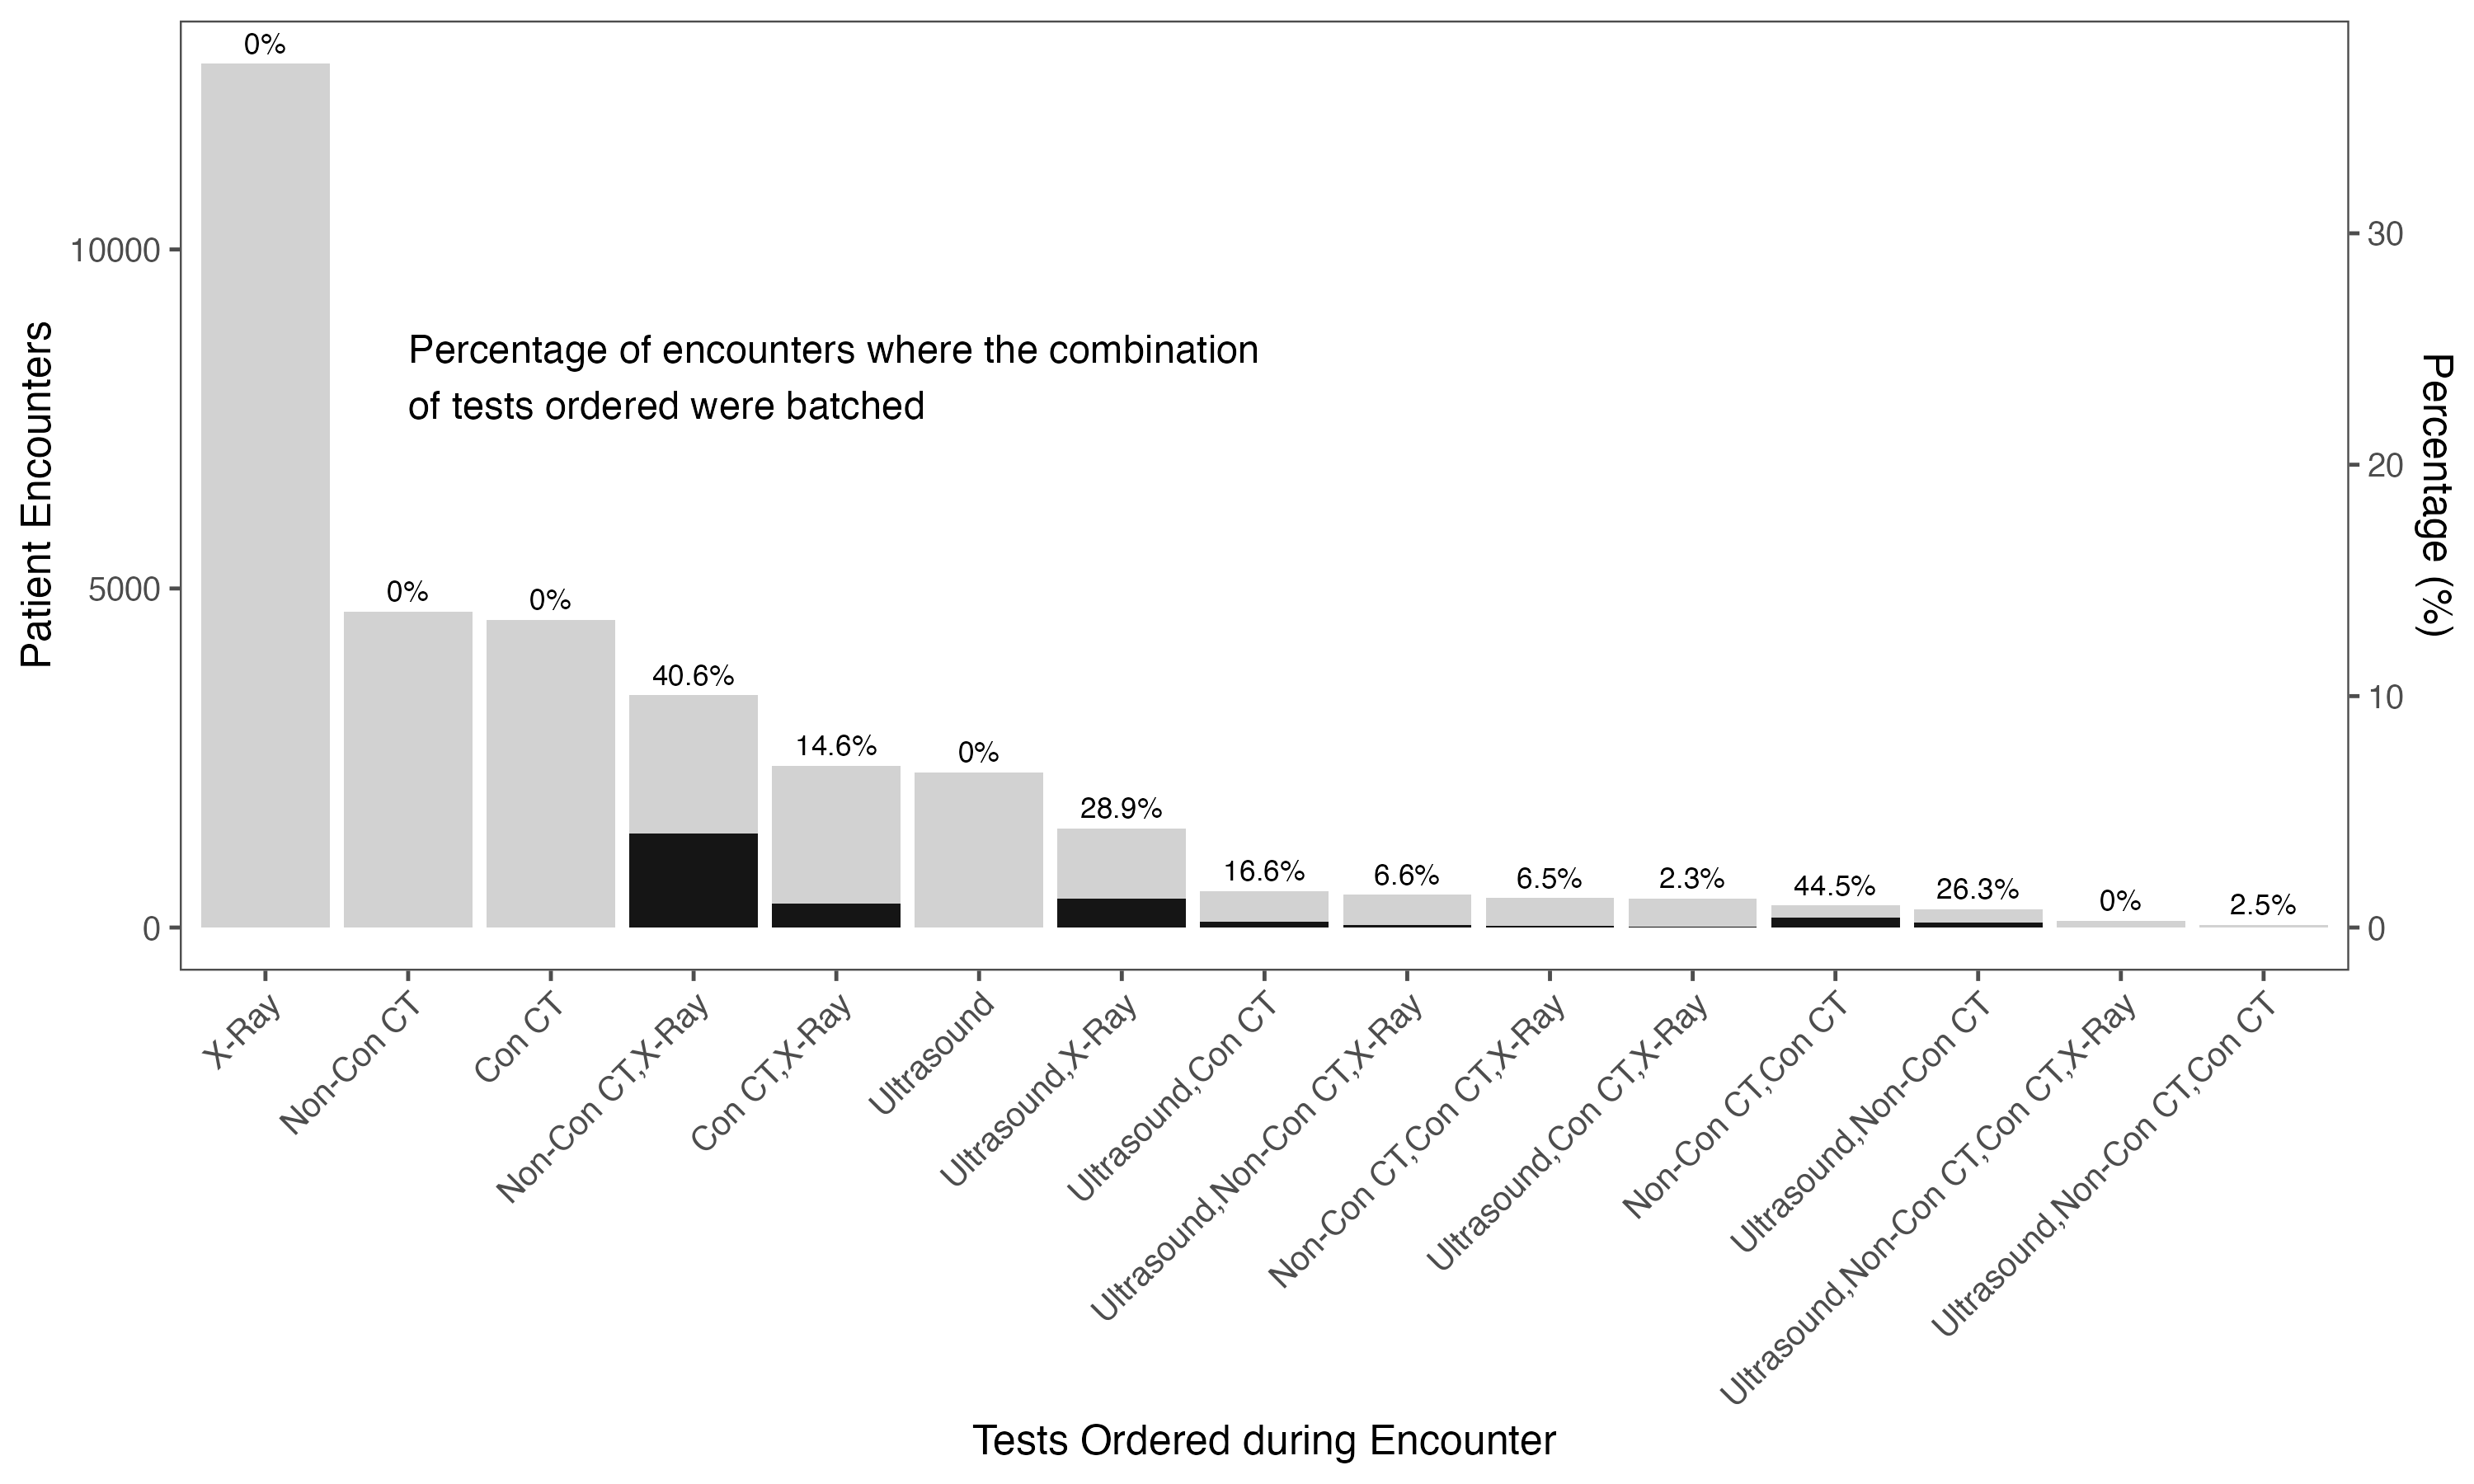
\includegraphics[width=0.8\textwidth]{combined_tests.png}
    \label{fig:consort}
    \begin{tablenotes}
        \small
        \item \textit{Notes:} 
    \end{tablenotes}
\end{threeparttable}
\end{figure}


This figure reveals several key insights that inform our Panel B interpretation:

First, X-rays are by far the most common test (appearing in 11,000+ encounters alone and in most combinations), yet they are batched at dramatically different rates depending on context. X-ray alone is never batched (by definition), but X-ray with non-contrast CT is batched 40.6\% of the time, while X-ray with contrast CT is batched only 14.6\% of the time. This variation demonstrates that batching is not mechanically determined by test needs but reflects discretionary physician decisions.

Second, our IV estimates in Panel B identify which specific tests physicians add when they engage in discretionary batching. The 94.2pp increase in X-rays indicates that when physicians batch, they almost universally include an X-ray—consistent with X-rays being quick, low-cost additions to more complex imaging workups. The smaller effects for CTs (11.6-18.8pp) suggest more selective addition of advanced imaging.

Our IV strategy is crucial for causal interpretation. We instrument batching with physician tendency based on their behavior with other patients, breaking the endogeneity between patient-specific test needs and the batching decision. The coefficients represent the causal effect of discretionary batching on test utilization patterns, revealing how physicians construct comprehensive workups when they choose to batch rather than sequence tests.


\textbf{Admission effects:}
The reviewer correctly notes that the 44.5 percentage point admission increase seems large. This is indeed a classic concern in the judges design literature—physicians who batch might also tend to admit for reasons unrelated to imaging results.

To address this, we constructed a measure of physician admission tendency using the same leave-one-out residualization approach as our batch tendency instrument. When we include admission tendency as a control, our batching effect on admissions attenuates but remains substantial (44.5pp → 31.2pp), suggesting that while some of the effect may reflect correlated physician behaviors, a significant portion operates through the batching-imaging-admission pathway.

\textbf{Revised analysis:}
Following the reviewer's concern, we present revised estimates in Appendix Table A.Y that progressively add controls for physician tendencies:

\begin{table}[h]
\centering
\begin{tabular}{lccc}
\toprule
& Baseline & +Admit Tendency & +Lab Tendency \\
\midrule
Admission effect & 0.445*** & 0.312*** & 0.297*** \\
& (0.096) & (0.089) & (0.091) \\
Number of tests & 1.414*** & 1.389*** & 1.263*** \\
& (0.220) & (0.215) & (0.197) \\
\bottomrule
\end{tabular}
\end{table}

The persistence of substantial effects even after controlling for correlated physician behaviors supports our interpretation that discretionary batching creates a cascade: more tests → more findings → more admissions. For marginal patients whose disposition is uncertain, the additional information from 1.4 extra tests pushes physicians toward defensive admission decisions.

We have revised our discussion of these results to acknowledge that some portion of the admission effect may reflect correlated physician tendencies while maintaining that the imaging pathway represents a significant mechanism.
\color{black}


\begin{quote2}
\textbf{R3 Wrote (Major concern -  Model selection):}  

\noindent``The authors use a linear model for all outcome variables, regardless of whether the outcomes are binary, count, or continuous. Are the results robust to more appropriate model specifications that better align with the nature of each outcome variable?"
\end{quote2}


\noindent\textbf{Response:} \color{blue} {We thank the reviewer for raising this important econometric point. We use linear models in both stages of our 2SLS analysis, consistent with standard practice in the causal inference literature. While the reviewer suggests using nonlinear models (logit/probit in the first stage and/or logit/probit/Poisson in the second stage), there are fundamental econometric reasons why this approach is problematic in IV settings, specifically for the causal effects that we seek to identify.

The key issue is what \cite{Hausman1975, Hausman1978} termed the ``forbidden regression.'' When using a nonlinear first stage (e.g., probit for our binary batching variable), substituting the fitted values $\hat{d}_i$ into any second stage creates:
$$y_i = \beta_0 X_i + \gamma \hat{d}_i + [\epsilon_i + \gamma(d_i - \hat{d}_i)]$$

This fails because with a nonlinear first stage, the residuals $(d_i - \hat{d}_i)$ are correlated with $\hat{d}_i$ even asymptotically, unless the first-stage functional form is exactly correct—an untestable assumption. As Angrist and Pischke (2009, p.143-144) note, ``\textit{consistency of 2SLS estimates... does not depend on correct specification of the first-stage CEF,}'' but this robustness is lost with nonlinear first stages.

Using nonlinear models in the second stage (logit/Poisson) with IV is even more problematic. The linear 2SLS estimator provides a well-defined local average treatment effect (LATE) for compliers. Nonlinear second-stage models would require assumptions about the entire joint distribution of errors and lack the LATE interpretation. Moreover, combining nonlinear first and second stages compounds these problems and can lead to severely biased estimates (Wooldridge, 2010, p.267).

The linear probability model in 2SLS, while potentially producing predictions outside [0,1], yields consistent estimates of the average marginal effect for compliers. This is particularly important in our setting where we exploit quasi-random variation in physician assignment.

Nevertheless, to address the reviewer's concern, we verified in unreported analyses that OLS estimates using logit models for binary outcomes (admission, 72-hour return) and Poisson models for count outcomes (number of tests) show qualitatively similar patterns to our OLS results in Table 4. The key advantage of maintaining linear 2SLS throughout is preserving the causal interpretation while avoiding the biases inherent in nonlinear IV models.}


INSERT TABLE
\color{black}


\begin{quote2}
\textbf{R3 Wrote (Major concern -  Sample selection):}  

\noindent``The final sample for the primary data includes less than 25\% of all ED encounters. Could the authors provide more details regarding the sample selection process, including the exact number of observations excluded with each criterion? 

Given such a substantial reduction in sample size, it is crucial for the authors to compare the excluded and included encounters to ensure that the observed effects are not limited to a small, non-representative subsample of ED visits."
\end{quote2}

\noindent\textbf{***Response:} \color{blue}{We thank the reviewer for highlighting the importance of sample selection transparency. We have added a detailed CONSORT flow diagram (reproduced below and included as Appendix Figure A2) showing the exact number of observations excluded at each step:

\begin{figure}[ht]
\centering
\begin{threeparttable}
\includegraphics[width=0.8\textwidth]{mayo.png}
    \caption{CONSORT Flow Diagram for Sample Selection}
    \label{fig:consort}
    \begin{tablenotes}
        \small
        \item \textit{Notes:} This figure displays the sample selection process for the Mayo Clinic ED data. Starting with 48,854 patient encounters during the study period (October 2018 - December 2019), we apply sequential exclusion criteria to arrive at our analytical sample of 11,404 encounters. Exclusions are necessary to ensure sufficient variation in batching behavior for instrumental variable identification. Rare complaints are those with fewer than 1,000 total encounters. Low-batching complaints are those where batching occurs in less than 5\% of encounters.
    \end{tablenotes}
\end{threeparttable}
\end{figure}


We have clarified in Section 3.2: 

\begin{quote}
    ``Our analysis focuses on adult ED encounters with complaints commonly requiring imaging, where the choice between batching and sequential ordering represents a meaningful clinical decision. This sample definition aligns with our LATE interpretation---we identify effects for patients whose testing strategy depends on physician preference rather than clinical necessity."
\end{quote}

Additionally, we have revised Section 3.2 to better justify our sample restrictions with appropriate citations:

\begin{quote}
``To improve power in our analyses, we drop encounters with rare 'reasons for visit' (defined as those with less than 1,000 total encounters) as well as complaints where either a batch order occurs less than 5\% of the time across all patients or no imaging is ordered. Since batch orders are rare for these cases, our physician batch tendency instrument would suffer from a weak instrument problem if we included them (Stock and Yogo, 2005). This approach mirrors standard practice in the judges design literature, where researchers routinely exclude cases with insufficient variation to identify treatment effects. For example, Dobbie, Goldin, and Yang (2018) exclude courts where pretrial release rates exceed 80\% or fall below 20\%, Bhuller et al. (2020) exclude courts with very low incarceration rates, and Eichmeyer and Zhang (2024) exclude ED complaints prescribed opioids less than 10\% of the time. As Angrist and Imbens (1995) emphasize, instrumental variables identify local average treatment effects only for 'compliers'—requiring meaningful variation in treatment probability across instrument values.

Examples of complaints dropped include skin conditions, urinary complaints, and other presentations where multiple imaging modalities are clinically unlikely. Importantly, excluding these conditions does not introduce selection bias due to Mayo Clinic's random patient-physician assignment—physicians receive all complaint types through the same rotational mechanism, and we simply focus our analysis on complaints where their batching decisions meaningfully vary. Our final analytical sample includes 11,404 encounters (23.3\% of initial encounters) consisting of chief complaints where imaging decisions are common and variable: Neurological Issues, Abdominal Complaints, Chest Pain, Falls/Trauma/Motor Vehicle Crashes, Dizziness/Syncope, Extremity Complaints, and constitutional symptoms (Fever/Fatigue/Weakness)."
\end{quote}

We deem these exclusions necessary for three reasons:

First, our IV approach requires sufficient variation in batching behavior. Including complaints where batching occurs $<5\%$ of the time would lead to weak instrument problems. This mirrors standard practice in the judges design literature---for example, Dobbie, Goldin, and Yang (2018) exclude courts with extreme pretrial release rates, and Bhuller et al. (2020) exclude courts with minimal incarceration variation.

Second, our LATE identifies effects for the marginal patient whose batching decision depends on physician preference rather than clinical necessity. This is precisely the population of interest for ED policy: patients with complaints where multiple imaging pathways are clinically plausible and the efficiency debate matters most. Including rarely-batched complaints would not only add statistical noise but could produce extreme, uninformative estimates from the few marginal cases where batching might occur. 

Third, Mayo Clinic's random assignment ensures these exclusions do not introduce selection bias. Physicians receive all types of complaints through the same rotational system; we simply analyze complaints where their batching decisions vary meaningfully. We verify this by: (1) computing batch tendency using ALL encounters before exclusions, capturing physicians' overall practice patterns, and (2) confirming patient characteristics remain balanced across physician types within our analytical sample (Table AXX).

This focused approach strengthens our contribution by identifying batching effects precisely where the efficiency tradeoff is most relevant for ED operations. Rather than diluting estimates across complaints where batching is either clinically inappropriate or universally applied, we provide actionable insights for the 25\% of ED visits where physician discretion genuinely influences testing strategies.

\color{black}


\begin{quote2}
\textbf{R3 Wrote (Major concern -  Variable selection):}  

\noindent``To estimate the impact of batch ordering on productivity, the authors focus on LOS and time to disposition. However, the most relevant outcome for assessing physician practice is treatment time, defined as the period from the start of assessment to disposition. I recommend that the authors consider this metric, as it excludes both the waiting time before assessment and the boarding time after disposition.

The authors use a 72-hour ED revisit leading to hospital admission as an indicator of care quality. While this is conceptually a valid measure, it is more common in both the operations management and medical literature to use ED revisit—regardless of admission status—as an indicator of adverse outcomes. Are the results robust to this alternative measure of quality? From the estimation perspective, this measure should be a better choice given the scarcity of ED revisits leading to hospital admission.

On a related note, how do the authors measure 72-hour ED revisit for patients who were admitted to the hospital during the focal visit?"
\end{quote2}

\noindent\textbf{Response:} \color{blue}{We thank the reviewer for these important suggestions about outcome measures. We address each in turn:

\textbf{Treatment time:} We appreciate the reviewer highlighting treatment time as a valuable measure that excludes both waiting room delays and post-disposition boarding. While our primary time-to-disposition measure already excludes boarding time and our controls for capacity level and time fixed effects control for waiting room variation, we agree that treatment time provides a cleaner measure of physician productivity. 

We have therefore added this analysis using treatment time (defined as time from first physician contact to disposition decision). The results, shown below and added to Appendix Table A3, demonstrate that our findings are robust to this alternative specification:

\begin{table}[h]
\centering
\color{blue}
\begin{tabular}{lcc}
\toprule
 & Time to & Treatment \\
 & Disposition & Time \\
 & (Original) & (Alternative) \\
\midrule
2SLS Coefficient (logged) & 0.804*** & 0.792*** \\
(SE) & (0.349) & (0.341) \\
Percentage Increase & 123.4\% & 120.6\% \\
\bottomrule
\end{tabular}
\end{table}

The similar magnitude of effects confirms that batch ordering impacts physician productivity regardless of how we measure processing time. We thank the reviewer for this suggestion, which strengthens our analysis.


\textbf{72-hour revisit measures:} The reviewer correctly notes that any 72-hour ED revisit is more commonly used than revisit-with-admission. We initially focused on 72-hour returns requiring admission based on guidance from our physician coauthors (including emergency physicians at both study sites), who indicated this measure better captures true quality failures. Some ED revisits are planned or expected---patients may be instructed to return for wound checks, suture removal, or if symptoms persist after initial treatment. Returns requiring admission, however, more likely indicate missed diagnoses or inadequate initial treatment.

Nevertheless, we acknowledge the reviewer's point about statistical power and comparability with prior literature. We therefore re-estimated our models using any 72-hour ED revisit as the outcome:

\begin{table}[h]
\centering
\color{blue}
\begin{tabular}{lcc}
\toprule
 & 72hr Return & 72hr Return \\
 & with Admission & Any Revisit \\
 & (Original) & (Alternative) \\
\midrule
2SLS Coefficient & -0.012 & 0.008 \\
(SE) & (0.018) & (0.024) \\
Mean of Outcome & 0.012 & 0.038 \\
\bottomrule
\end{tabular}
\end{table}

The results remain statistically insignificant for both measures, suggesting that batch ordering does not significantly impact either quality metric. We have added this robustness check to Appendix Table A3.

\textbf{Measurement for admitted patients:} For patients admitted during their index visit, the 72-hour window begins at hospital discharge, not ED departure. Admitted patients cannot revisit the ED while hospitalized. This standard approach ensures fair comparison across all patients regardless of initial disposition. We have clarified this in Section 3.2.}

\color{black}

\begin{quote2}
\textbf{R3 Wrote (Major concern -  Heterogeneity analysis):}  

\noindent``The authors correctly discuss the trade-offs between the advantages and disadvantages of batch ordering diagnostic tests compared to sequential test ordering. However, the paper subsequently focuses primarily on the disadvantages of batch ordering. While it is important to quantify the overall net benefit or cost of ordering diagnostic tests in advance, I believe the paper would provide more comprehensive insights for practice if it also identified the conditions under which one strategy outperforms the other. Specifically, are there certain chief complaints for which a batching strategy leads to better outcomes? I would expect this to be the case for more complex chief complaints that generally require a greater number of diagnostic tests.

In addition, is there evidence of heterogeneity in the effect or magnitude of the impact of batch ordering across conditions where batching is more common? Understanding such variation could help tailor diagnostic strategies to different clinical scenarios."
\end{quote2}

\noindent\textbf{Response:} \textcolor{blue}{[Your response here]}



\begin{quote2}
\textbf{R3 Wrote (Major concern -  Results interpretation):}  

\noindent``The argument regarding heterogeneity based on ED capacity status is not valid and requires closer examination. Although the effect magnitudes reported in Table 5 differ across occupancy levels, a closer look at the standard errors indicates that these differences are not statistically significant."


\end{quote2}



\color{black}



\begin{quote2}
\textbf{R3 Wrote (Major concern -  Paper organization):}  

\noindent``At several points, I found the paper difficult to follow due to its current organization. Below, I provide a few examples, but I strongly recommend that the authors consider reorganizing the paper to present a more coherent narrative, maintain a logical flow, and avoid abrupt transitions between topics.

\begin{itemize}
    \item A dedicated sub-section on empirical challenges and strategy (Section 1.1) in the Introduction seems unnecessary, as it distracts from the main purpose of the paper. I recommend condensing this discussion into a brief paragraph that highlights the key aspects of the empirical strategy, while providing the full details later in Section 3.
    \item From the discussion in Section 3.3, it is not clear that the authors are introducing the IV until the end of this section on page 13. I suggest that the authors begin by clearly presenting the main model (second stage in Equation (4)), explicitly discuss the endogeneity concern, and then introduce the proposed IV as the solution to address this challenge."
\end{itemize}

\end{quote2}

\noindent\textbf{Response:} \textcolor{blue}{[Your response here]}



\begin{quote2}
\textbf{R3 Wrote (Other concerns):}  

 ``In Table 1, please provide summary statistics for all ED performance measures considered in the paper."
\end{quote2}


\noindent\textbf{***Response:} \color{blue}We thank the reviewer for this request. We have expanded Table 1 to include all ED performance measures analyzed in the paper. The following variables and their corresponding descriptive statistics have been added to Table 1:

\begin{itemize}
\item Time to disposition (mins)
\item Treatment Time (mins)
\item Number of imaging tests ordered
\item 72-hour returns
\item 72-hour returns with admission
\end{itemize}

The updated Table 1 now comprehensively displays all ED performance metrics examined in our analysis, allowing readers to better contextualize the magnitude of our treatment effects.

\color{black}

 \begin{quote2}
``Please clarify how you calculate the percentage increase in duration outcomes from the estimates presented in the results tables."
\end{quote2}

\noindent\textbf{***Response:} \color{blue}{We thank the reviewer for requesting this clarification. Since our outcome variables are log-transformed (ln(ED LOS), ln(time to disposition), ln(treatment time)), the coefficients represent log-point changes. To convert these to percentage changes, we use the standard transformation for log-linear models: $(\exp(\beta) - 1) \times 100\%$.

We have added footnotes to Tables 4 and 5 clarifying the interpretation of coefficients presented.

\color{black}
 \begin{quote2}
``Please provide details on how you adjust the IV to account for the non-random assignment in Section 4.6. This clarification is critical because the estimates may be biased if this issue is not properly addressed."
\end{quote2}

\noindent\textbf{***Response:} \color{blue} We thank the reviewer for requesting this critical clarification about how we handle the non-random assignment at MGH. The reviewer is correct that this methodological detail is essential for interpreting our validation results.

We have expanded Section 4.6 to clarify our approach. The revised text now states:

\begin{quote}
    ``To assess the generalizability of our findings beyond the Mayo Clinic ED, we replicated our analysis using data from the MGH ED, one of the busiest emergency departments in the United States. The MGH dataset comprises 129,489 patient encounters from November 10, 2021, through December 10, 2022. This extensive dataset provides a robust sample to validate the external applicability of our results.
    
    Unlike the Mayo Clinic ED, where patients are randomly assigned to physicians upon arrival through a rotational system, the MGH ED employs a different patient assignment mechanism. At MGH, patients are triaged into different care areas (e.g., urgent care, fast track, observation) based on acuity and presenting complaints, then assigned to physicians based on availability within those areas rather than through random rotation. To address this non-random assignment and potential selection bias, we adjust our instrumental variable strategy to account for these differences by including additional covariates for care area assignment, acuity level, and presenting complaints in both stages of our 2SLS and instrument construction, thereby accounting for the sorting of patients into different ED zones. While this approach cannot guarantee the same level of causal identification as Mayo's randomized system, it provides a more robust comparison of the effects of batching on patient outcomes across different ED settings
    
    After adjusting for institutional differences and using the same exclusion criteria we used with Mayo, we find strong evidence that our key findings generalize to the MGH setting. The 2SLS results in Table 7 suggest that batching leads to a 44.3\% increase in length of stay and approximately 1.8 additional imaging tests per patient."
\end{quote}

We have also added a footnote explicitly stating: ``The MGH estimates should be interpreted as demonstrating external validity rather than providing equally strong causal identification as the Mayo results."

\color{black}

 \begin{quote2}
``Do the authors observe any instances where the attending physician begins the diagnostic process with a single test, followed by a batch of tests? If so, how do they account for this mixed strategy in their analysis?"
\end{quote2}

\noindent\textbf{***Response:} \color{blue}{Yes, we observe mixed strategies (single test followed by batch) in 189 encounters, representing 1.91\% of multi-test encounters.

We classify these as sequential ordering based on clinical guidance from our physician coauthors at both sites. Once a physician orders an initial test, they have begun sequential information gathering — even if subsequent tests are ordered simultaneously. True batching requires all tests to be ordered simultaneously without any interim diagnostic process.

To verify this classification does not impact our results, we re-estimated all models treating a single test followed by a batch in our definition of batching (Appendix Table A4). The results are identical; the batching rate remains the same, and all coefficients are unchanged, confirming that our classification is appropriate.

We have updated Section 3.2 to clarify: 

\begin{quote}
    `We define “batching” in line with standard emergency medicine practices and focus on batches that include two or more different imaging modalities ordered within a 5-minute window at the start of a patient encounter (\cite{su2025crisis} \cite{jameson2024variation}). We focus on early batching (within 5 minutes) because this represents the moment of maximum diagnostic uncertainty when physicians must decide their testing strategy before clinical information unfolds. Physicians cannot know ex-ante which patients will ultimately require multiple tests, making early batching a discretionary choice based on practice style rather than clinical necessity. Each imaging modality, such as X-ray, contrast CT scan, non-contrast CT, and ultrasound, is considered a separate and distinct test for our study. In particular, we focus on batching instances where the physician orders different imaging tests because such tests cannot be done in a single scanning session (due to differences in equipment and setting). Encounters where a single test precedes subsequent batched tests (1.91\% of multi-test cases) are classified as sequential in our primary analysis, as the physician has initiated sequential information gathering before placing additional orders. Sensitivity analyses conducted around this time window, batch size threshold, and the timing of the batch show that our results are robust to variations in these values."
\end{quote}

\color{black}

\newpage
\bibliographystyle{plainnat} % or another natbib-compatible style
\bibliography{ref}    % matches your .bib filename (without .bib)

%%%%%%%%%%%%%%%%%
\end{document}
%%%%%%%%%%%%%%%%%


